\documentclass[12pt, a4paper, tocpage=plain]{abnt} % Fonte tamanho 12, papel A4, páginas do sumário sem o p.<número da página>

\usepackage[utf8]{inputenc} % Dá suporte para caracteres especiais como acentos e cedilha
\usepackage[brazil]{babel} % Gera datas e nomes em português com estilo brasileiro
\usepackage{hyperref} % Permite a criação de hyperlink no documento, como os links usados na referência
\usepackage[alf]{abntcite} % Define o estilo de referência bibliográfica
\usepackage{graphicx} % Permite a utilização de imagens no documento
\usepackage[small]{caption} % Define as legendas das figuras com fontes menores do que o texto
\usepackage{pslatex} % Define que o formato da letra será Times New Roman
\usepackage{epigraph} % Permite a criação de epígrafes 
\usepackage{setspace} % Permite a definição de espaçamento entre linhas
\usepackage[top=3cm, left=3cm, right=2cm, bottom=2cm]{geometry} % Define as margens da folha
\usepackage{listings}
\lstset{language=C++,
		stepnumber=1,
		firstnumber=1,
		numberstyle=\tiny,
		extendedchars=true,
		breaklines=true,
		frame = shadowbox,
		basicstyle=\footnotesize,
		stringstyle=\ttfamily,
		showstringspaces=false,
		literate={--}{--}1
}
\hyphenpenalty=5000
\tolerance=1000
\sloppy
 
\setcounter{secnumdepth}{3} % Até três subsubsections numeradas
\setcounter{tocdepth}{3} % Até trẽs subsubsections numeradas

\setlength{\parindent}{1.25cm} % Define o recuo da primeira linha dos parágrafos para 1.25 cm

\renewcommand{\ABNTchapterfont}{\bfseries} % Define a fonte do \chapter
\renewcommand{\ABNTchaptersize}{\large} % Define o tamanho da fonte do \chapter
\renewcommand{\ABNTsectionfontsize}{\large} % Define o tamanho da fonte da \section
\renewcommand{\ABNTsubsectionfontsize}{\large} % Define o tamanho da fonte do \subsection
\renewcommand{\ABNTsubsubsectionfontsize}{\large} % Define o tamanho da fonte do \subsubsection
\renewcommand{\ABNTbibliographyname}{REFERÊNCIAS BIBLIOGRÁFICAS} % Modifica o título gerado pelo \bibliographys

\begin{document} % Começo do TCC
\begin{titlepage}
 \begin{figure}[ht]
 \centering
 \scalebox{0.35}{
\includegraphics{figuras/logo}}
 \end{figure}
 \begin{center}
   {\large CURSO DE BACHARELADO SISTEMAS DE INFORMAÇÃO} \\ [3.5cm]
  	{\large CHAIANA LAYZA DO NASCIMENTO} \\
	{\large FELIPE DA SILVA FERREIRA} \\	
	{\large GABRIEL NASCIMENTO MARCOS DA ROCHA} \\ [4cm]
   {\large SERVIDOR LINUX COM SAMBA - PDC (PRIMARY DOMAIN CONTROLLER). COMPARTILHAMENTO DE ARQUIVOS, IMPRESSORAS E CONTRALADOR DE DOMÍNIO EM MAQUINAS WINDOWS.}\\ [2cm]
   \vfill
   {\large Campos dos Goytacazes/RJ} \\
   {\large 2012}
 \end{center}
\end{titlepage}
 % Cria a capa
\begin{titlepage}
 \begin{figure}[ht]
 \centering
 \scalebox{0.35}{
\includegraphics{figuras/logo}}
 \end{figure}
 \begin{center}
   	{\large CURSO DE BACHARELADO SISTEMAS DE INFORMAÇÃO} \\ [3.5cm]
	{\large CHAIANA LAYZA DO NASCIMENTO LIMA} \\
	{\large FELIPE DA SILVA FERREIRA} \\	
	{\large GABRIEL NASCIMENTO MARCOS DA ROCHA} \\ [4cm]
   	%{\large SAMBA 3 E ACTIVE DIRECTORY COM SAMBA 4.}\\ [2cm]
   	{\large SAMBA 3 E 4 COMO CONTROLADOR DE DOMÍNIO, SERVIDOR DE ARQUIVOS E DE IMPRESSÃO: UMA ALTERNATIVA LIVRE PERANTE AS SOLUÇÕES PROPRIETÁRIAS.}\\ [2cm]
   \hspace{.45\textwidth} % posicionando a minipage
   \begin{minipage}{0.5\textwidth}
   \begin{espacosimples}
        Trabalho de conclusão de curso apresentado ao Instituto Federal Fluminense como requisito parcial para conclusão do Curso de Bacharelado em Sistemas de Informação.\\[1.5cm]
        Orientador: Prof. Vinicius
    \end{espacosimples}
    \end{minipage}
   \vfill
   {\large Campos dos Goytacazes/RJ} \\
   {\large 2012}
 \end{center}
\end{titlepage}
 % Cria a folha de rosto
\begin{folhadeaprovacao}
    \setlength{\ABNTsignthickness}{0.4pt}
    \setlength{\ABNTsignwidth}{15cm}
    \setlength{\ABNTsignskip}{0.9cm}
    \begin{center}
	{\large CHAIANA LAYZA DO NASCIMENTO LIMA} \\
	{\large FELIPE DA SILVA FERREIRA} \\	
	{\large GABRIEL NASCIMENTO MARCOS DA ROCHA} \\ [2cm]
%	{\large SAMBA 3 E ACTIVE DIRECTORY COM SAMBA 4.}\\ [2cm]
	{\large SAMBA 3 E 4 COMO CONTROLADOR DE DOMÍNIO, SERVIDOR DE ARQUIVOS E DE 	IMPRESSÃO: UMA ALTERNATIVA LIVRE PERANTE AS SOLUÇÕES PROPRIETÁRIAS.}\\ [0.5cm]
        \hspace{.45\textwidth} % posicionando a minipage
        \begin{minipage}{0.5\textwidth}
        \begin{espacosimples}
        Trabalho de conclusão de curso apresentado ao Instituto Federal Fluminense como requisito parcial para conclusão do Curso de Bacharelado de Sistema de Informação.\\\\
        \end{espacosimples}
        \end{minipage}
    \end{center}
    Aprovada em  de 22 Novembro de 2012 \\\\
    Banca avaliadora:
    \assinatura{Prof. Vinicius Barcelos da Silva (Orientador) \\ Mestre em Engenharia de Produção / UENF \\ Instituto Federal de Educação, Ciência e Tecnologia Fluminense}
    \assinatura{Prof. Fernando Luiz de Carvalho e Silva \\	Mestre em Engenharia de Produção / UENF \\ Instituto Federal de Educação, Ciência e Tecnologia Fluminense}
    \assinatura{Prof. José Elias da Silva Justo \\ Mestre em Pesquisa Operacional e Inteligência Computacional / UCAM-CAMPOS \\ Instituto Federal de Educação, Ciência e Tecnologia Fluminense}
 	\assinatura{Prof. Rogério Avelar \\ Mestre em Pesquisa Operacional e Inteligência Computacional / UCAM-CAMPOS \\ Instituto Federal de Educação, Ciência e Tecnologia Fluminense}
\end{folhadeaprovacao}
 % Cria a folha de aprovação
\null
\vfill

{\normalsize \it \hfill Aos nosso amigos, professores e familiares , \vspace*{4pt}

\hfill com amor\dots}
  % Cria a folha de dedicatória
\begin{center}
\textbf{AGRADECIMENTOS}
\end{center}

Queremos agradecer a Deus, pois sem ele nada seria possível, nossas famílias que nos apoiam em todas decisões, nossos colegas de trabalho que sempre nos ajudam e ao IFF por nos proporcionar recursos financeiros e materiais para o desenvolvimento deste trabalho.
 % Cria a folha de agradecimentos
\null % o \vfill só funciona com o \null
\vfill
\epigraph{Integração Contínua é uma atitude, não uma ferramenta.}{James Shore}
 % Cria a epígrafe (onde se coloca um pensamento)
\begin{center}
\textbf{RESUMO}
\end{center}
\singlespacing

\noindent 
	O objetivo deste trabalho foi desenvolver uma ferramenta que possa identificar os metadados de um arquivo PDF com formatação de artigo, respeitando da norma ABNT, (título, palavras-chave, autor, etc.) e utilizá-los para renomear o arquivo de modo a facilitar seu reconhecimento, visando uma maior organização e distinção do mesmo.
 \\
\noindent PALAVRAS-CHAVE: Metadados, PDF, Extração de dados, Desenvolvimento de Software
%Com o avanço da tecnologia, é cada vez mais comum a disponibilização de conteúdo acadêmico (artigos, trabalhos de conclusão de curso, teses, etc.) na internet para fins de pesquisa. Grande parte desses documentos é encontrada em formato PDF (Portable Document Format), por ser um formato largamente conhecido e muito utilizado para leitura de arquivos em tela, preservando sua qualidade e formatação independentemente do computador ou do sistema operacional utilizado.
 % Tendo em vista esse grande volume de documentos disponíveis, é comum que não haja uma preocupação por parte de seus autores em nomeá-los de acordo com o título do conteúdo ou com o assunto abordado. Baixar um arquivo com nome incompatível com seu conteúdo não seria problema se esse arquivo não se misturasse a vários outros em mesma situação no disco de armazenamento do usuário, o que fatalmente acontece. % Resumo do trabalho
\begin{center}
\textbf{ABSTRACT}
\end{center}

\singlespacing

\noindent This work suggests a proposal to implement a files and printers sharing server and a domain controller in an educational institution, with mission to facilitate the sharing of available network
resources, making safer and reliable the control of user’s access to these resources. More specifically, this work implements the open source Samba, in versions 3 and 4, as a free alternative to 
proprietary solutions such as Microsoft Active Directory, serving the resources above both Windows and Linux clients. Will also be presented basic concepts for the understanding of the tools 
used in addition to step-by-step instructions and scripts needed to carry out the implementation of the entire structure proposed in this work.\\

\noindent KEYWORDS: Linux, Samba, PDC, Share, LDAP, Active Directory % Resumo em língua estrangeira
\renewcommand{\listfigurename}{LISTA DE FIGURAS} % Modifica o nome da lista de figuras
\listoffigures % Gera o índice de figuras
\listoftables % Gera o índice de tabelas
\renewcommand{\contentsname}{SUMÁRIO} % Modifica o nome do sumário
\tableofcontents % Gera o sumário
\onehalfspacing % Define o espaçamento de 1.5cm entre linhas
\chapter{INTRODUÇÃO}

  Com o avanço da tecnologia, é cada vez mais comum a disponibilidade de conteúdo acadêmico (artigos, trabalhos de conclusão de curso, teses, etc.) na internet para fins de pesquisa. Grande parte desses documentos é encontrada em formato PDF (Portable Document Format), por ser um formato largamente conhecido, muito utilizado para leitura de arquivos e com fácil criação a partir de outros documento (DOC, ODT,PPT, entre outros) preservando sua qualidade e formatação independentemente do computador ou do sistema operacional utilizado.

 Os artigos em pdf gerados são armazenados geralmente em servidores acadêmicos ou em sistemas genéricos de armazenamento e na maioria das vezes sem preocupar com a melhor indexação dos mesmos, com isso acaba
acarretando em armazenar um arquivo com nomes sem significados para os humanos. ex:  o código do arquivo no banco de dados no servidor. Nomes sem significados complica a organização dos arquivos em computadores
pessoais quando são armazenados em grande escala, pois é difícil distinguir os temas, autores e títulos.


%A atual conjuntura econômica mundial configura um ambiente de extrema competição, onde os mecanismos de diferenciação se interagem, condicionando o desempenho das empresas em seus respectivos mercados. Nesse contexto, a busca da eficiência e eficácia é uma exigência que se impõe a todos os processos e níveis organizacionais presentes nas atividades produtivas. Para não perderem suas fatias de mercado, as empresas tendem a se posicionar mais agressivamente nessa disputa. Nesse caso, a grande organização muitas vezes leva vantagem por estar mais bem estruturada.

%À medida em que a competição se torna mais acirrada, maior é a importância dos ganhos de produtividade trazidos pela tecnologia da informação. Essa tendência influencia toda a cadeia produtiva, o que faz prever que qualquer empresa, independente de seu porte ou tipo de atividade, terá que considerar os impactos que seus softwares trarão para seus negócios, seu mercado e sua concorrência. As empresas estão utilizando cada vez mais os softwares como ferramenta de competitividade, com impactos importantes e positivos nos seus negócios, nos mais variados ramos de atividade.

%Percebeu-se que com a mudança constante do mercado ou até mesmo nas próprias empresas, os softwares precisam acompanhar estas mudanças, com a maior rapidez possível, garantindo assim qualidade, mantendo confiabilidade, eficiência e escala de produção. Controlar a qualidade de sistemas de software é um grande desafio devido à alta complexidade dos produtos e às inúmeras dificuldades relacionadas ao processo de desenvolvimento, que envolve questões humanas, técnicas, burocráticas, de negócio e políticas. Idealmente, os sistemas de software devem, não só fazer corretamente o que o cliente precisa, mas também fazê-lo de forma segura, eficiente, escalável, flexível e de fácil manutenção e evolução \cite{OLIVEIRA}. Com isso, surge a idéia dos testes automatizados, que fazem com que o custo e o risco do software caiam consideravelmente, aumentando a confiabilidade, pois com estes o desenvolvedor tem certeza que o software faz exatamente o que deveria fazer \cite{MYERS}. A grande vantagem desta abordagem, é que todos os casos de teste podem ser facilmente e rapidamente repetidos a qualquer momento e com pouco esforço.

%A reprodutibilidade dos testes permite simular identicamente, e quantas vezes for desejada, situações específicas, garantindo que passos importantes não sejam ignorados por falha humana, facilitando a identificação de um possível comportamento não desejado \cite{DELAMARO}.

%Além disso, como os casos para verificação são descritos através de um código interpretado por um computador, é possível criar situações de testes bem mais elaboradas e complexas do que as realizadas manualmente, possibilitando qualquer combinação de comandos e operações \cite{DELAMARO}. Utilizando testes automatizados, é possível simular centenas de usuários acessando um sistema ou inserir milhares de registros em uma base de dados, o que não é factível com testes manuais.

%Todas estas características ajudam a solucionar os problemas encontrados nos testes manuais, diminuindo a quantidade de erros e aumentando a qualidade do software. Como é mais rápido e fácil executar todos os testes a qualquer momento, mudanças no sistema podem ser feitas com segurança, o que aumenta a vida útil e qualidade do produto. Com isso surgiu a idéia da Integração Contínua, que consiste em uma prática em que os desenvolvedores de uma equipe integram seu trabalho pelo menos uma vez por dia, o que consequentemente levará a múltiplas integrações do sistema \cite{FOWLER}, facilitando assim a detecção de erros inesperados \cite{DUVALL}.

\section{Justificativa do trabalho}

   A ferramenta de extração de metadados de PDF foi escolhida como tema deste trabalho, pois oferece uma maneira mais rápida de distinguir artigos e organiza-los em pastas e por não ter muitas ferramentas no mercado.

% A Integração Contínua foi escolhida como tema deste trabalho por se tratar de uma técnica recente, com poucas referências teóricas que abordam especificamente o assunto. Além disso, o desejo de criar um material que se torne uma referência, em português, para que outras pessoas possam estudar sobre o assunto.

\section{Objetivo}

O principal objetivo deste trabalho é, através de um estudo de caso, documentar e implantar a Integração Contínua em um projeto real. Almeja-se, também, fornecer ao leitor deste trabalho, conhecimento técnico sobre a aplicação dos conceitos da Integração Contínua. Desta forma, deseja-se descrever estes conceitos para equipes de desenvolvimento de software que vislumbram os benefícios desta técnica. Ademais, aumentar a confiabilidade do projeto da Biblioteca Digital da RENAPI, visando um projeto mais robusto e menos suscetível a erros.

\section{Estrutura do trabalho}

Este trabalho se divide em 5 capítulos e está estruturado da seguinte maneira:

No capítulo 2 é feita uma fundamentação de conceitos e técnicas necessárias para o entendimento deste trabalho.

No capítulo 3 é feita uma descrição da Integração Contínua, seus componentes, suas práticas e suas vantagens.

Já no capítulo 4, é apresentado um estudo de caso, em que os autores deste trabalho são responsáveis por implantar um ambiente de Integração Contínua, em um projeto real de desenvolvimento de software.

E por fim, o capítulo 5 apresenta os resultados obtidos com o estudo de caso bem como os trabalhos futuros a serem desenvolvidos no processo da Integração Contínua implantado no projeto.
 % Cria o capítulo 1
\chapter{TECNOLOGIAS DISCUTIDAS}

Este capitulo faz uma introdução das tecnologias utilizadas, tais como o Samba, NetBIOS, \textit{Active Directory}, DNS, LDAP, Kerberos, entre outros, além da apresentação de termos técnicos essenciais para o melhor entendimento deste trabalho.

\section{Samba}

Samba é um \textit{software} \textit{open source} que provê serviços a clientes utilizando os protocolos SMB e CIFS.

SMB, que significa Server Message Block, é um protocolo de compartilhamento de arquivos, impressoras, portas seriais, e abstrações de comunicação, tais como pipes nomeados e slots de correio entre computadores.\cite{SMB}

O protocolo CIFS foi um renomeamento da Microsoft de futuras versões do SMB que foram usados nos produtos Window - os dois termos podem ser usados indistintamente. \cite{SAMBA}

O samba permite a interoperabilidade entre servidores Linux/Unix e clientes baseados na
plataforma Windows.
O samba permite que um servidor Linux seja apto a fornecer serviços como:
  \begin{itemize}
    \item \textbf{Servidor de arquivos e impressão} - Utilizando o protocolo \textit{Server Message Block} para possibilitar o compartilhamento de arquivos, pastas volumes e impressoras na rede, com um controle de permissões de acessos a usuários e grupos juntamente com as permissões locais atribuídas as pastas compartilhadas. Algumas permissões de acesso local serão explicadas no tópico sobre permissões especiais no Linux.

    \item \textbf{Autenticação e autorização} - Identifica um computador ou um usuário da rede e determina os direitos de acesso a arquivos que cada usuário possui, através de tecnologias como permissões de arquivos, diretivas de grupo e o serviço de autenticação Kerberos.

    \item \textbf{Resolução e busca de nomes e diretórios} - Compartilha as principais informações sobre computadores e usuários da rede através do \textit{LightWeight Directory Access Protocol} (LDAP).% e o Microsoft Active Directory.

    \item \textbf{Servidor de domínio como PDC} - Funcionando como controlador de domínio ativo dentro de um domínio Windows. Para melhor entendimento ele será explicado no tópico sobre PDC.
  \end{itemize}

Basicamente, o Samba é um servidor e um conjunto de ferramentas que permite o compartilhamento de arquivos e impressoras em sistemas Windows e Linux. Outra característica do Samba é poder atuar como um Controlador Primário de Domínio (PDC), armazenando perfis de usuários e realizar controle de acesso. \cite{FOCA}.

\section{PDC (Primary Domain Controller)}

O Controlador de Domínio é responsável por fornecer autenticação para os clientes, sejam sistemas Linux ou Windows. Ou seja, apenas centraliza contas de usuários e fornece recursos voltados para a administração de usuários, como a gestão de perfis móveis, que são as configurações de usuários que são lidas, independente de qual máquina o usuário utilize. Em uma rede com mais de 10 clientes a necessidade de ter um PDC é mais aparente, pois fica cada vez mais difícil gerenciar as contas de clientes e máquinas conforme o crescimento da mesma. Com o Controlador de Domínio também é possível fornecer acesso por perfis móveis onde o usuário pode ter acesso à sua área de trabalho independente da máquina (da mesma rede) onde faz o login. Em contrapartida, bloqueando uma conta de usuário,automaticamente este estará bloqueado em todas as máquinas gerenciadas pelo Controlador de Domínio \cite{MORIMOTO}

\section{Permissões especiais no Linux}

Existe no Linux três permissões especiais, para dar segurança ao sistema, chamadas assim por somente serem atribuídas a arquivos específicos (arquivos executáveis e diretórios). Tais permissões são fornecidas pelos bits SUID, SGID e STICKY.

  \begin{itemize}
    \item \textbf{SUID} - O bit SUID (Set UID) é aplicável apenas a arquivos executáveis, fazendo com que estes rodem com as permissões de seu proprietário, independente de quem tenha executado-o. Pode ser útil para que usuários comuns possam executar arquivos permitidos apenas a administradores.

    \item \textbf{SGID} - O bit SGID (Set GID) pode ser aplicado a um arquivo executável e a um diretório. No primeiro caso ele tem as mesma função do SUID, porém rodando com as permissões de um grupo de usuários. No segundo, ele força os arquivos e diretórios criados dentro do diretório pai (o que obteve a permissão) a pertencerem ao mesmo grupo, independente do grupo de quem o tenha criado.

    \item \textbf{STICKY} - O bit STICKY é aplicável a diretórios e faz com que a exclusão de arquivos pertencentes a estes diretórios seja apenas permitida ao dono do arquivo e ao administrador do sistema. Tem vantagem sobre a permissão “Somente Leitura” no diretório pois faz com que outros usuários possam criar e editar qualquer arquivo, impedindo-os apenas de apagá-lo.
  \end{itemize}

É importante ressaltar que de nada adiantará se os arquivos e diretórios possuírem uma determinada permissão local, e esta ser diferente da permissão configurada no Samba. Por exemplo: de nada adiantará atribuir acesso de escrita a um arquivo no Linux se ele possui permissão ``Somente Leitura" no Samba. A atribuição mais negativa, ou seja, a que concede menos permissões (neste caso a ``Somente Leitura") prevalecerá sobre a outra.

\section{NETBIOS}

Um nome NetBIOS é um endereço de 16 bytes usado para identificar um recurso NetBIOS na rede. Um nome NetBIOS é um nome único (exclusivo) ou de grupo (não exclusivo). Quando um processo de NetBIOS está comunicando-se com um processo específico em um computador, é usado um nome exclusivo. Quando um processo de NetBIOS está comunicando-se com vários processos em vários computadores, é usado um nome de grupo. A resolução de nomes NetBIOS significa o mapeamento bem-sucedido de um nome NetBIOS para um endereço IP.\cite{NETBIOS}

O NetBIOS trabalha na camada sessão do modelo OSI (\textit{Open Systems Interconnection}), e utiliza as portas de comunicação UDP (\textit{User Datagram Protocol}) 137 e 138 para a resolução dos NetBios \textit{names} e \textit{datagrams} e 139 de comunicação TCP (\textit{Transmission Control Protocol}) para NetBios \textit{sessions}, conforme a Figura \ref{netbios}

\begin{figure}[ht]
   	\centering
    \scalebox{1}{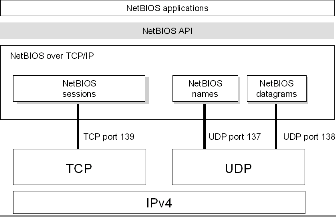
\includegraphics{figuras/netbios}}
   	\caption{Estrutura do funcionamento da NetBios \cite{NETBIOS}}
    \label{netbios}
\end{figure}

\section{\textit{Active Directory}}

O \textit{Active Directory} (AD) é um serviço de diretório nas redes a partir do Windows 2000.

Serviço de diretório é um conjunto de atributos sobre recursos e serviços existentes na rede, isso significa que é uma maneira de organizar e simplificar o acesso aos recursos da rede, centralizando-os; bem como, reforçar a segurança e dar proteção aos objetos da base de dados contra intrusos, ou controlar acessos dos usuários internos da rede.

O \textit{Active Directory} mantém dados como contas de usuários, impressoras, grupos, computadores, servidores, recursos de rede, etc. Ele pode ser totalmente escalonável, aumentando conforme a necessidade.\cite{LOSANO}

\section{LDAP}

O LDAP (\textit{Lightweight Directory Access Protocol}) é o protocolo responsável por fornecer Serviço de Diretórios a computadores Windows de forma similar ao \textit{Active Directory} da Microsoft, que é baseado no LDAP. Tais serviços incluem conexões de computadores, grupos de computadores, usuários, administração de identidades, além de possibilitar uma maneira eficiente de descrever, localizar e administrar esses recursos. Essa estrutura do LDAP pode ser vista na Figura \ref{ldap}

LDAP é um protocolo para acessar informações contidas em um diretório. Por ser um protocolo cliente/servidor o LDAP permite navegar, ler, armazenar e pesquisar informações e realizar tarefas de gerenciamento em um serviço de diretórios. O serviço de diretório é um banco de dados otimizado para leitura, navegação e pesquisas \cite{TRIGO}.

\begin{figure}[ht]
   	\centering
    \scalebox{1}{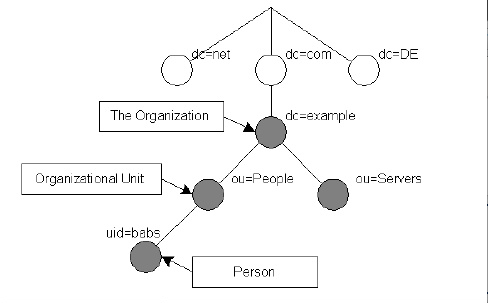
\includegraphics{figuras/ldap}}
   	\caption{Estrutura do protocolo LDAP \cite{LDAP}}
    \label{ldap}
\end{figure}

\section{DNS}

DNS (\textit{Domain Name System}) é uma base de dados hierárquica e distribuída, usada para a resolução de nomes de domínios em endereços IP (\textit{ Internet Protocol}). É considerado como um banco de dados distribuído que converte nomes de \textit{hosts} (máquinas) para endereços IP. É basicamente um mapeamento de endereços IP e seus respectivos nomes. A utilização mais comum é na internet. Todos os computadores da rede possuem um endereço IP. Os servidores DNS simplesmente transformam ou resolvem esse número em um nome \cite{SCRIMER}. Por exemplo, o endereço www.iff.edu.br corresponde ao IP 200.143.198.110. Exemplos de domínios DNS que podem ser visto na Figura \ref{dns}

\begin{figure}[ht]
   	\centering
    \scalebox{1}{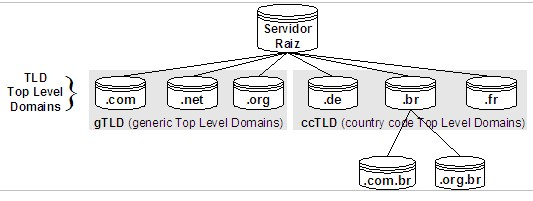
\includegraphics{figuras/servidor_dns}}
   	\caption{Estrutura hierárquica do DNS \cite{DNS}}
    \label{dns}
\end{figure}

\section{BIND}

BIND é um \textit{software} de código livre que implementa o Sistema de Nomes de Domínio (DNS) de protocolos para a internet. É uma referência em implementação desses protocolos, mas também possui uma produção em série de \textit{software}, adequado para uso em aplicações de alto volume e de alta confiança. O BIND está disponível para \textit{download} gratuito sob os termos da Licença ISC, um estilo de licença BSD. \cite{BIND}.

\section{Kerberos}

Kerberos é um protocolo de segurança de rede e fornece autenticação entre computadores e usuários através de um servidor centralizado que concede autenticações criptográficas a qualquer computador utilizando o Kerberos. Esse sistema de segurança e autenticação agrega diversos benefícios como autentificação mútua, autentificação delegada, interoperabilidade e gerência simplificada e confiável. O samba pode usar o Kerberos como um mecanismo autenticação de computadores e usuários.

O Kerberos é um protocolo que prevê forte autenticação entre aplicações cliente-servidor e usa criptografia de chave simétrica no qual servidores fornecem acesso aos serviços solicitados pelos clientes, caso provem que são eles mesmos. \cite{FILHO}

 
\begin{figure}[ht]
   	\centering
    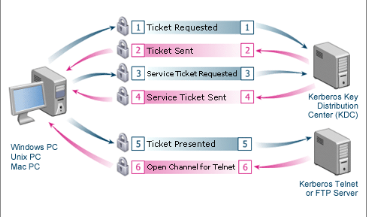
\includegraphics[width=0.9 \textwidth]{figuras/kerberos} 
   	\caption{Autenticação Kerberos \cite{KERBEROS}}
    \label{kerberos}
\end{figure}

%\pagebreak
 
%\section{NTP}

%Os servidores NTP permitem aos seus clientes a sincronização dos relógios de seus computadores e outros equipamentos de rede a partir de uma referência padrão de tempo aceita mundialmente, conhecida como UTC (\textit{Universal Time Coordinated}).\cite{RNP}

%\section{NTVFS}

%Sistema de arquivos que armazena os atributos do NTFS

\section{GSSAPI}

A GSSAPI é uma interface que permite aos desenvolvedores escreverem aplicações que aproveitam mecanismos de segurança tais como Kerberos, sem ter de programar explicitamente para qualquer mecanismo, ou seja, aplicações genéricas do ponto de vista de segurança. Programas que usam GSSAPI são, deste modo, altamente portáteis, não somente de uma plataforma para outra, mas de uma configuração de segurança a outra e de um protocolo de transporte a outro. A GSSAPI fornece vários níveis de proteção de dados, consistentes com os mecanismos de segurança subjacentes.\cite{HUGO} % Cria o capítulo 2 
\chapter{SAMBA 3}
Este capítulo descreve como são feitas a instalação e a configuração de um servidor Samba 3 como controlador de domínio, servidor de impressão e servidor de arquivos, respeitando as regras de usuários e permissões.

\section{Instalação do Samba 3}

O pacote Samba 3 pode ser instalado através do repositório de sistemas da distribuição Linux na qual será configurado (neste trabalho foram utilizadas as distribuições Ubuntu 11.04 e Debian 6.0.5). Antes da instalação é necessário atualizar a base de dados do repositório para que possa instalar a versão mais atual do Samba 3.
 
\begin{enumerate}
    \item \textbf{\# apt-get update} - Atualiza a base de dados do repositório no Ubuntu.
    \item \textbf{\# apt-get install samba} - Realiza a instalação do pacote Samba 3.
    \item \textbf{\# apt-get install smbclient} - Pacote que mostra as informações do servidor Samba 3 e permite acesso de compartilhamentos no windows ou linux a partir de uma máquina linux.
\end{enumerate}

\section{SWAT - Gerenciando o Samba 3 pelo browser}

O SWAT é uma ferramenta para a edição do /etc/smb.conf, porém por meio de uma interface gráfica. Com ele é possível compartilhar impressoras, arquivos, criar usuários, permitir ou restringir acessos.

\begin{enumerate}
 \item \textbf{\# apt-get install swat} - Instala a ferramenta gráfica SWAT para o gerenciamento do Samba 3.
    \item \textbf{\$ firefox localhost:901} - Endereço de acesso no \textit{browser} (neste caso o Firefox) para acessar o SWAT.
\end{enumerate}

Ao acessar o SWAT pelo navegador, o usuário deve informar o usuário root e sua senha. Após o login no sistema, pode-se observar na barra de ferramentas as opções de configuração do SWAT, conforme Figura \ref{swat}. A função de cada opção é detalhada a seguir:

\begin{figure}[ht]
   	\centering
    \scalebox{1}{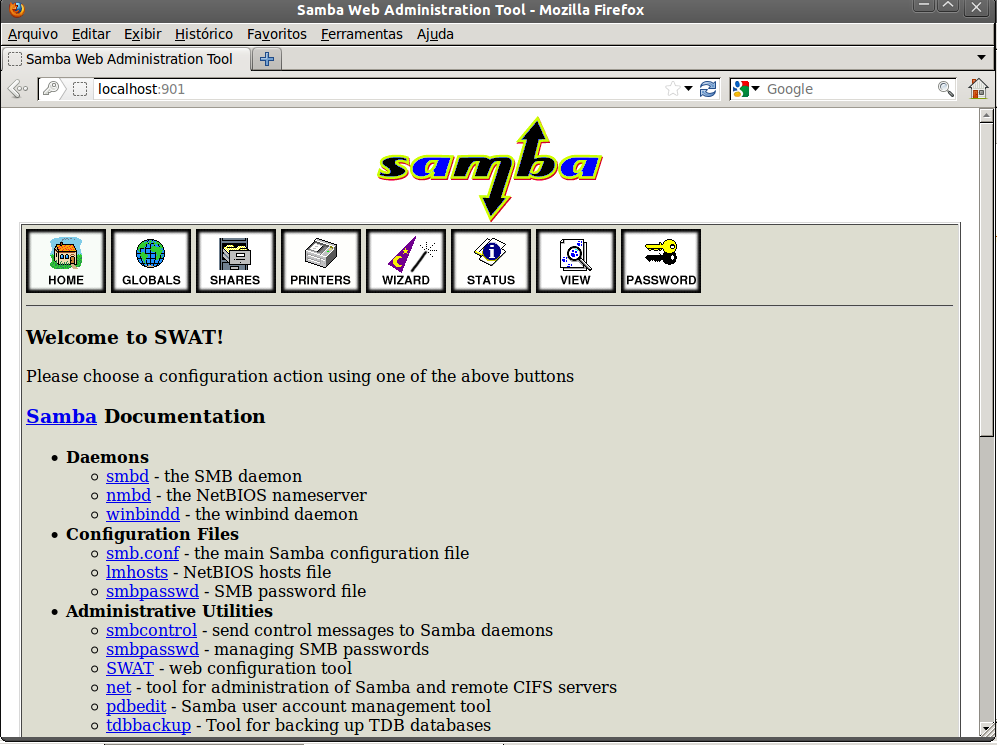
\includegraphics{figuras/swat}}
   	\caption{Tela do SWAT}
    \label{swat}
\end{figure}

\begin{itemize}
    \item \textbf{Home} - Documentação do Samba 3
    \item \textbf{Globals} - Variáveis globais de configuração do Samba 3
    \item \textbf{Shares} - Ativar compartilhamentos de diretórios e arquivos
    \item \textbf{Printers} - Compartilhamento de impressoras
    \item \textbf{Wizard} - Escreve as modificações no arquivo smb.conf do Samba 3
    \item \textbf{Status} - Status do servidor com usuário, compartilhamento dos ativos e arquivos abertos
    \item \textbf{View} - Mostra o arquivo smb.conf
    \item \textbf{Password} - Cadastrar o usuário, máquinas e mudar senha dos usuários no servidor
\end{itemize}

Por se tratar de uma ferramenta gráfica o SWAT torna mais fácil a edição e adição de configurações no smb.conf, mas toda vez que as configurações são alteradas e salvas ele gera um novo arquivo smb.conf e com isso apaga todos os possíveis comentários existentes no arquivo. Por se tratar de um arquivo com muitas variáveis, parâmetros e seções, nesse trabalho o foco será a edição através de editores de texto padrão como o ``vim", pois assim algumas configurações podem ser inseridas como comentários para fins de explicação ou como base para futuras modificações.

\section{Iniciando Samba 3}

Com todos os componentes instalados a aplicação pode ser iniciada. O Samba 3 trabalha com dois \textit{daemon} principais, geralmente eles se encontram no /usr/sbin/,  que são: SMBD e o NMBD

O SMBD permite compartilhamento de arquivos e impressoras em uma rede SMB e provê autorização e autenticação a usuários SMB. O NMBD cuida do \textit{Windows Internet Name Service} (WINS) e auxilia com a navegação e resolução de nomes.\cite{SAMBA}

Existem varias formas de iniciar e parar os processos do Samba 3, que como:
\begin{itemize}
	\item \textbf{\# /etc/init.d/smbd start} - Inicia o Samba 3. 
	\item \textbf{\# service smbd start} - Inicia o Samba 3.
	\item \textbf{\# service smbd stop} - Para o processo do Samba 3.
%	\item \textbf{\# service smbd restart} - Finaliza o processo existente e cria outro para o Samba 3.
	\item \textbf{\# /etc/init.d/samba start} - Para iniciar o Samba 3 em computadores com Debian 6.
	%\item \textbf{\# /etc/init.d/samba stop} - Para o Samba 3 no Debian 6.
\end{itemize}

\section{Seções}

No Samba 3, as configurações de compartilhamentos, impressoras e gerais, são realizadas através de um único arquivo de configuração, o ``/etc/samba/smb.conf". Esse arquivo para melhor organização, fica dividido em sessões, sendo a primeira sessão nomeada como [global], onde são definidas as configurações gerais do servidor. Também podem ser criadas sessões adicionais para cada compartilhamento, sendo nomeadas com o nome do mesmo. Se for necessário criar um compartilhamento com o nome ``arquivo", a sessão que deve ser criada no arquivo de configuração deve ser [arquivo].

\section{Variáveis de substituição do Samba 3}

Existem variáveis especiais que podem ser usadas no arquivo de configuração do Samba 3 e são substituídas por parâmetros especiais no momento da conexão do usuário \cite{FOCA}. Um exemplo de utilização de variáveis de substituição seria mudar a localização do diretório home do usuário conforme no Quadro \ref{variavel_home}:\\

\begin{lstlisting}[caption=Exemplo de utilização das variáveis de substituição,label={variavel_home}]	
[home]
	
comment = Diretorio home do usuario

path = /home/usuarios/%u
\end{lstlisting}          

Ao longo deste trabalho diversas variáveis de substituição serão utilizadas, principalmente nos scripts aqui propostos. Cada uma das variáveis são descritas em detalhes a seguir:

\%S - O nome do serviço atual, se existir. Seu uso é interessante, principalmente no uso de diretórios homes.

\%P - O diretório raíz do serviço atual, se existir.

\%u - O nome de usuário do serviço atual, se aplicável. Esta variável é bastante útil para programação de scripts e também para criar arquivos de log personalizados, etc.

\%g - O grupo primário do usuário \%u.

\%U - O nome de usuário da seção (o nome de usuário solicitado pelo cliente, não é uma regra que ele será sempre o mesmo que ele recebeu).

\%G - O nome do grupo primário de \%U.

\%H - O diretório home do usuário, de acordo com \%u.

\%v - A versão do Samba.

\%h - O nome DNS da máquina que está executando o Samba.

\%m - O nome NetBIOS da máquina do cliente. Isto é muito útil para log de conexões personalizados e outras coisas úteis.

\%L - O nome NetBIOS do servidor. Como o servidor pode usar mais de um nome no Samba (aliases), você poderá saber com qual nome o seu servidor está sendo acessado e possivelmente torna-lo o nome primário de sua máquina.

\%M - O nome DNS da máquina cliente.

\%N - O nome do seu servidor de diretórios home NIS. Este parâmetro é obtido de uma entrada no seu arquivo auto.map. Se não tiver compilado o SAMBA com a opção --with-automount então este valor será o mesmo de %L.

\%p - O caminho do diretório home do serviço, obtido de uma entrada mapeada no arquivo auto.map do NIS. A entrada NIS do arquivo auto.map é dividida na forma ``\%N:\%p".

\%R - O nível de protocolo selecionado após a negociação. O valor retornado pode ser CORE, COREPLUS, LANMAN1, LANMAN2 ou NT1.

\%d - A identificação de processo do processo atual do servidor.

\%a - A arquitetura da máquina remota. Somente algumas são reconhecidas e a resposta pode não ser totalmente confiável. O Samba atualmente reconhece Samba, Windows for Workgroups, Windows 95, Windows NT e Windows 2000. Qualquer outra coisa será mostrado como \textit{``UNKNOWN"} (desconhecido).

\%I - O endereço IP da máquina do cliente.

\%T - A data e hora atual.

\%\$(var\_ambiente) - Retorna o valor da variável de ambiente especificada.

\section{Configuração do Samba para ser um PDC}

O arquivo de configuração se encontra no diretório /etc, onde está a maioria dos arquivos de configuração dos programas no linux.

\begin{enumerate}
	\item \textbf{\# cp /etc/samba/smb.conf /etc/samba/smb.conf.bkp} - Por motivo de segurança é recomendado fazer um backup do arquivo. Ele contém exemplos comentados das possíveis configurações do Samba 3, auxiliando o profissional de TI no momento de sua configuração.
	\item \textbf{\# testparm -s /etc/samba/smb.conf.bkp $>$ /etc/samba/smb.conf} - Removerá os comentário para melhor leitura do arquivo. Observação: o arquivo de origem não pode ser o smb.conf pois ele irá se rescrever e o arquivo só conterá a seção [global] vazia.  
	\item \textbf{\# gedit /etc/samba/smb.conf} - Para editar o arquivo e adicionar as seções, parâmetros e variáveis.
\end{enumerate}

Agora é necessário inserir, modificar e remover alguns parâmetros na seção [global] para que o Samba 3 se comporte como um PDC. Conforme o Quadro \ref{smb_global}\\

\begin{lstlisting}[caption=Exemplo do que deve ser inserido no smb.conf,label={smb_global}]
[global] 

workgroup = 'nome do servidor de domnio'

server string = 'Titulo'       

security = user

netbios name = 'nome que sera da netbios do servidor'

domain master = yes

domain logons = yes

enable privileges = yes

passdb backend = tdbsam
	
encrypt passwords = true

preferred master = yes

local master = yes

os level = 100

map to guest = Bad User

panic action = /usr/share/samba/panic-action \%d	
\end{lstlisting}

Explicação das variáveis utilizadas:

\begin{itemize}
	\item \textbf{workgroup} - Nome do servidor de domínio.
	\item \textbf{server string} - Descrição do servidor que aparece na barra de título das janelas do compartilhamento.
	\item \textbf{security} - Tipo de segurança do compartilhamento. Existem os tipos domain, user e share.
		\begin{enumerate}
			\item {share}  - É utilizado quando o compartilhamento será aberto, onde todos os usuários conectados serão guest e sem a necessidade de realizar login.
			\item {user} - Todos os usuários que tentarem se conectar terão que se identificar por meio de um login e uma senha.
			\item {domain} - Quando um servidor de domínio será responsável pela identificação e segurança dos usuários.
		\end{enumerate} 
	\item \textbf{netbios name} - Nome da netbios do servidor.
	\item \textbf{encrypt passwords} - Quando informado o valor ``true" as senhas informadas para o servidor serão criptografadas.
	\item \textbf{domain master} - Informa que o servidor Samba 3 será o domínio principal da rede.
	\item \textbf{domain logons} - O servidor Samba 3 passa a ser um controlador de domínio.
	\item \textbf{enable privileges} - Habilita alguns privilégios no Samba 3. Alguns deles:
		\begin{enumerate}
			\item {SeAddUsersPrivilege} - Adicionar usuários e grupos no domínio 
			\item {SeDiskOperatorPrivilege} - Gerencia os discos compartilhados 
			\item {SeMachineAccountPrivilege} - Adicionar maquinas no domínio 
			\item {SePrintOperatorPrivilege} - Gerencia as impressoras
		\end{enumerate}
	\item \textbf{passdb backend} - Aceita valores smbpasswd ou tdbsam . Define qual será a forma de armazenagem dos registros dos usuários.
		\begin{enumerate}
			\item{smbpasswd} - O smbpasswd é o backend mais simples. Nele, as senhas são salvas no arquivo ``/etc/samba/smbpasswd" e são transmitidas de forma encriptada através da rede, com suporte ao sistema NTLM, usado pelas versões contemporâneas do Windows. A vantagem do smbpasswd é que ele é um sistema bastante simples. Embora encriptadas, as senhas são armazenadas em um arquivo de texto, com uma conta por linha.\cite{BACKEND}
			\item{tdbsam} - O tdbsam usa uma base de dados muito mais robusta, armazenada no arquivo ``/var/lib/samba/passdb.tdb".\cite{BACKEND}
			\item{Diferença entre smbpasswd e tdbsam} - O tdbsam oferece duas vantagens sobre o smbpasswd: oferece um melhor desempenho em servidores com um grande número de usuários cadastrados e oferece suporte ao armazenamento dos controles SAM (\textit{Software Asset Management}) estendidos usados pelas versões server do Windows. O uso do tdbsam é fortemente recomendável caso seu servidor tenha mais do que algumas dezenas de usuários cadastrados ou caso você pretenda usar seu servidor Samba como PDC da rede. Ele é também um pré-requisito caso você precise migrar um domínio NT já existente para o servidor Samba. \cite{BACKEND}
		\end{enumerate}
	\item \textbf{local master} - Define se o servidor será o \textit{Master Browser}.
	\item \textbf{os level} - Valor que será passado na eleição para definir o mestre da rede. O valor máximo é 100, assim vencendo os valores padrões de ``os level" o servidores windows.
%	\item \textbf{win support} - Se nmbd será um servidor WINS.
	\item \textbf{map to guest} - Torna usuário guest todos que não conseguirem se identificar com um login e senha valida.
	\item \textbf{panic action} - Comando que será executado caso o smbd ou nmbd parem de funcionar.
\end{itemize}

Com todas as variáveis devidamente adicionadas o servidor Samba 3 precisa ser reiniciado para que todas as modificações entrem em vigor.

\begin{enumerate}
	\item \textbf{\# testparm} - Verifica se existe algum erro de sintaxe no arquivos de configuração no smb.conf. Exemplo de execução que pode ser visto na Figura \ref{testparm}
	\item \textbf{\# /etc/init.d/smbd restart} - Reinicia o Samba 3.
	\item \textbf{\# /etc/init.d/nmbd restart} - Reinicia o servidor de nomes do Samba 3.
\end{enumerate}

\begin{figure}[ht]
   	\centering
    \scalebox{1}{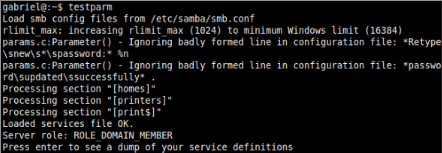
\includegraphics{figuras/testparm}}
   	\caption{Saída do testparm}
    \label{testparm}
\end{figure}

\section{Cadastro de Usuário}

Os usuários que terão acesso e permissões de login no domínio devem ser criados no servidor linux, onde se encontra o Samba 3. O usuário root tem que ser cadastrado no Samba 3 antes de qualquer outro usuário, pois ele é o administrador da aplicação.

\begin{itemize}
	\item \textbf {\# smbpasswd -a root} - Uma senha terá que ser informada e precisa ser a mesma do usuário no sistema.
\end{itemize}

Cada usuário no sistema deverá conter uma pasta com o nome de ``profile.pds". Essa pasta irá conter informações das sessões de \textit{logon} que o usuário fez no servidor de domínio. Para automatizar a criação dessa pasta no diretório \textit{home} dos usuários, cria-se o diretório no /etc/skel.

\begin{itemize}
	\item \textbf{\# mkdir /etc/skel/profile.pds} - O /etc/skel armazena todos os diretórios e arquivos que serão criados juntos com o usuário no sistema.
\end{itemize}

Antes de cadastrar os usuários no Samba 3 eles precisam ser criados no sistema.

\begin{itemize}
	\item \textbf{\# adduser "--disabled-login usuario} - Comando para a criação mais completa de usuário no linux com nome completo, telefone e outros dados, porém sem a permissão de login e entre outros dados.
\end{itemize}

Após o usuário ser criado no sistema, ele necessita ser cadastrado no Samba 3.

\begin{itemize}
	\item \textbf{\# smbpasswd -a usuario} - Informe a mesma senha cadastrada no linux.
\end{itemize}

\section{Cadastro de Máquinas}

Da mesma forma que os usuário têm que ser cadastrados no sistema, as máquinas que poderão entrar no domínio também devem ser cadastradas. As máquinas são cadastradas como usuários normais no linux antes de serem cadastradas no Samba 3, porém sem pasta home e sem bash para login.

\begin{enumerate}
	\item \textbf{\# groupadd machine} - Cria o grupo no qual serão adicionadas as máquinas cadastradas para melhor organização dos usuários no linux.
	\item \textbf{\# useradd "--home /dev/null "--shell /bin/false "--disabled-login "--group machine computador1\$} - 	Comando para a criação da máquina no sistema linux. Por padrão se adiciona o \$ no final do nome pois é dessa forma que o Samba 3 irá identificar que o usuário na verdade é uma máquina. 
	\item \textbf{\# passwd -l computador1\$} - Desativa a mudança da senha para o usuário/máquina.
\end{enumerate}

Após a criação do usuário/máquina no sistema agora ele tem que ser cadastrado no Samba 3.

\begin{itemize}	
	\item \textbf{\# smbpasswd -a -m computador1\$} - Cadastra a máquina no Samba 3.
\end{itemize}


\section{Script de Cadastro de Usuários e Máquinas}

Para facilitar a criação e exclusão dos usuários no sistema e no Samba 3, foi feito o script \textbf{smbmanager.sh}\footnote[1]{Pode ser baixado em https://github.com/GabrielRocha/Monografia/blob/master/latex/Scripts/smbmanager.sh} conforme o anexo no Apêndice A1. Com ele é possível criar usuários e máquinas, adicionar usuários em grupos e também excluí-los do sistema.

O script tem que ter a permissão de root para que possa ser iniciado.

\begin{enumerate}
	\item \textbf{\# chmod +x smbmanger.sh} - Adiciona a permissão de execução ao script.
	\item \textbf{\# cp smbmanager.sh /usr/sbin/} - Transferindo o script para a pasta /usr/sbin/ o script poderá ser iniciado em qualquer caminho que o usuário esteja.
	\item \textbf{\# ./smbmanager.sh} - Execução do \textit{script}. Figura \ref{smbmanager}
\end{enumerate}

\begin{figure}[ht]
   	\centering
    \scalebox{1}{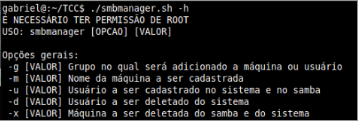
\includegraphics{figuras/smbmanager}}
   	\caption{Saída do smbmanager}
    \label{smbmanager}
\end{figure}

\section{Migração dos Usuários Administradores e Users do Linux para o Windows}

Para que o Windows possa reconhecer um grupo de usuários administradores do linux como Power Users e Domain Users deve se mapear os grupos pelo RID dos mesmos. A Tabela \ref{tab} apresenta alguns dos grupos e seus respectivos RID (\textit{Relative Identifier}). Os comandos a seguir devem ser utilizados para mapear esses grupos no Samba 3.

\begin{table}[h!]
	\centering
	\caption{Tabela do RID (\textit{Relative Identifier}) Windows \cite{RID}}
	\begin{tabular}{cccc}
		
		\hline
		
		Well-Known Entity & RID & Type &	Essential \\
		
		\hline
		
		\hline
		
		Domain Administrator & 500 & User & No \\
		Domain Guest & 501 & User & No \\		
		Domain KRBTGT & 502	& User & No \\
		Domain Admins & 512 & Group & Yes \\
		Domain Users & 513 & Group & Yes \\
		Domain Guests & 514 & Group & Yes \\
		Domain Computers & 515 & Group & No \\
		Domain Controllers & 516 & Group & No \\
		Domain Certificate Admins & 517 & Group & No \\
		Domain Schema Admins & 518 & Group & No \\		
		Domain Enterprise Admins & 519 & Group & No \\
		Domain Policy Admins & 520 & Group & No \\
		Builtin Admins & 544 & Alias & No \\
		Builtin users & 545 & Alias & No \\
		Builtin Guests & 546 & Alias & No \\
		Builtin Power Users & 547 & Alias & No \\
		Builtin Account Operators & 548 & Alias & No \\
		Builtin System Operators & 549 & Alias & No \\
		Builtin Print Operators	& 550 & Alias & No \\
		Builtin Backup Operators & 551 & Alias & No \\
		Builtin Replicator & 552 & Alias & No \\
		%Builtin RAS Servers & 553 & Alias & No \\
		 	
		\hline
	\end{tabular}
	\label{tab}
\end{table}

\clearpage

\begin{itemize}
	\item \textbf{\# net groupmap list} - Liste os grupos existentes mapeados, caso não tenha o grupo siga os passos a seguir.
\end{itemize}
\begin{enumerate}
	\item \textbf{\# net groupmap add ntgroup=`Domain Admins' rid=512 unixgroup=admin} - Irá mapear o grupo admin para o grupo Domain Admins do windows.
	\item \textbf{\# net groupmap add ntgroup=`Domain Users' rid=513 unixgroup=users} - Mapea o grupo users com o Domain Users do windows.
\end{enumerate}

\begin{enumerate}
	\item \textbf{\# net groupmap delete ntgroup=`Domain Admins'} - Caso queira remover um mapeamento de grupo.
	\item \textbf{\# net groupmap modify ntgroup=`Domain Admins' rid=512 unixgroup=admin} - Caso tenha necessidade de modificar um mapeamento.
\end{enumerate}

Dessa forma, se o usuário logar com os usuários que estejam no grupo admin em algum terminal windows no domínio, ele terá permissões de administrador.

\section{Perfis Móveis}

Para que as configurações e personalizações do perfil do usuário no windows sejam salvas é necessário a criação de um perfil móvel no servidor Samba 3. 
A vantagem de se utilizar um perfil móvel é que não existe a obrigatoriedade de se realizar backup na máquina do usuário, pois os arquivos são salvos no servidor, sendo assim é só o usuário fazer o login em outra máquina windows que o seu perfil e os seus dados serão migrados para o novo computador. Porém o perfil móvel tem um problema que é a quantidade de dados armazenados. Se o número de usuários e dados de cada um for muito grande, cria-se a necessidade de ter um servidor com muito espaço de armazenamento e uma rede muito bem estruturada. 

Para ativar a configuração de perfil móvel no Samba 3 deve-se adicionar no [global] as variáveis mostradas no Quadro \ref{logon_path} \\

\begin{lstlisting}[caption=Variáveis necessárias para o perfil móvel,label={logon_path}]	
logon path = \\%L\Profiles\%U

logon home = \\%L\Profiles\%U

logon drive = H:	
\end{lstlisting}


\begin{enumerate}
	\item \textbf{logon path} - Serve para indicar o caminho onde vão ficar os perfis no Windows XP/Vista/7 
	\item \textbf{logon home} - Indica o caminho para os perfis em versões mais antigas do Windows, como 95/98.
	\item \textbf{logon drive} -  Unidade que será mapeada com o caminho $\backslash$$\backslash$servidor$\backslash$profiles$\backslash$"nome do usuário" no Windows.
\end{enumerate}

No exemplo apresentado, o diretório profile criado fica compartilhado para que seja mapeado na unidade H do usuário no windows.

Após a definição dessas três opções na seção [global], deve-se criar uma seção [profiles] contendo alguns comandos que serão detalhados a seguir no Quadro \ref{smb_profile}.\\

\begin{lstlisting}[caption=Variáveis para criação do compartilhamento profile,label={smb_profile}]	
[profiles] 

path = /var/samba/%U 
	
writeable = yes 
	
browseable = no 
	
create mask = 0600 
	
directory mask = 0700 
	
available = yes
	
\end{lstlisting}

\begin{itemize}
	\item \textbf {path} - Caminho da pasta que vai ser compartilhada.
	\item \textbf {writeable} - Permite a escrita no diretório e nos arquivos.
	\item \textbf {browseable} - Define se o compartilhamento poderá ser visto na pasta principal do compartilhamento ou somente pelo endereço completo.
	\item \textbf {create mask} - Força a criação dos arquivos com a permissão 0600, assim somente os donos do arquivo poderão alterar os arquivos.
	\item \textbf {directory mask} - Criação dos diretórios com permissão 0700.
	\item \textbf{available} - (Yes/No) Se o compartilhamento estará acessível ou não no servidor.
\end{itemize}

\section{Compartilhamento de Arquivos}

O compartilhamento de arquivos é dado pela adição de seções no arquivo smb.conf. Como pode ser visto no Quadro \ref{smb_diretoria}\\

\begin{lstlisting}[caption=Criação de uma seção para compartilhamento de arquivos,label={smb_diretoria}]
[Diretoria]

path = /media/diretoria

read only = no

valid users = +diretoria

force group = diretoria

create mask = 0770

directory mask = 0770

browseable = no
	
\end{lstlisting}

\begin{itemize}
	\item \textbf{[Diretoria]} - Nome do compartilhamento que será mostrado no servidor.
	\item \textbf{path} - Nele devemos mapear diretórios que serão compartilhados na rede. 
\end{itemize}

	Cabe ressaltar que após a criação desses diretórios, é necessário o ajuste das permissões de acesso, do dono do diretório e do grupo do diretório, utilizando os programas chmod e chown, respectivamente. O ajuste varia caso a caso, e deve ser realizado com cautela, para não dar mais permissões que o necessário. Uma breve explicação sobre o chmod e chown é realizada a seguir:

\# chmod - Define as permissões do arquivo. Exemplo: \# chmod 774 -R /pasta\_criada - essas permissões definem que o usuário proprietário do diretório e todos os usuário do grupo do diretório terão controle total no diretório e em seus arquivos e que os outro usuário poderão apenas listar os arquivos que se encontram no diretório.

\# chown - Define qual será o usuário e grupo proprietário do diretório ou arquivo. Exemplo: \# chown usuario.grupo /diretorio .

\begin{itemize}
	\item \textbf{read only} - Define se o compartilhamento estará com permissão de somente leitura ou não.
	\item \textbf{Valid users} - Define quais usuários e grupos poderão acessar o compartilhamento. O símbolo de + define que o nome inserido esta se referindo a um grupo de usuários.
	\item \textbf{force group} - Força qual será o grupo proprietário dos arquivos criados no compartilhamento.
	\item \textbf{create mask} - Permissão dos arquivos que forem criados ou inseridos no compartilhamento
	\item \textbf{directory mask} - Permissão dos diretórios criados dentro do diretório compartilhados.
	\item \textbf{browseable} - Define se o compartilhamento poderá ser visualizado na janela do compartilhamento do servidor.
\end{itemize}

Existem outras variáveis que podem ser adicionadas em um compartilhamento de arquivos dependendo da necessidade.

\begin{itemize}
	\item \textbf{invalid users} - Lista de usuários e grupos que não terão acesso.
	\item \textbf{guest ok} - Permite que qualquer usuário acesse a pasta.
	\item \textbf{veto files} - Impede que certos arquivos sejam transferidos para o servidor.
	\item \textbf{write list} - Lista dos usuários que poderão gravar e fazer alterações nos arquivos e diretórios compartilhados.
	\item \textbf{read list} - Lista dos usuários que só poderão ler e listar os arquivos e diretórios compartilhados.
	\item \textbf{host deny} - Ip`s ou faixa de ips que não podem conectar ao servidor.
	\item \textbf{hosts allow} - Ip`s ou faixas de ips que podem conectar ao compartilhamento.
\end{itemize}

\textbf{Aplicação de algumas das variáveis citadas acima que podem ser vista no Quadro \ref{smb_variavel}}\\

\begin{lstlisting}[caption=Aplicação de algumas variáveis no Samba 3,label={smb_variavel}]
[Backup]

write list = usuario1 # Somente o usuario1 tera permissao de escrita no compartilhamento.

read list = usuario2 # O usuario2 so podera ler e listas os arquivos e diretorios desse compartilhamento.

host allow = 192.168.1.2-192.168.1.20 # Somente os ip's que estiverem entre 192.168.1.2 e 192.168.1.20 poderao acessar esse compartilhamento.

veto files = *.tmp/*.doc # Nao sera permitido inserir esses tipos de arquivos no compartilhamento. Essa variavel aceita expressoes regulares
\end{lstlisting}

\section{Script Logon}

Para que os mapeamentos de unidades e alguns códigos sejam executados de forma automática nos usuários logados o Samba 3 fornece a opção na seção [global]. 

\begin{itemize}
	\item {logon script = \%G.bat } - Com essa variável adicionada, o sistema irá buscar o script com o nome do grupo primário do usuário. Trabalhar com o grupo é mais fácil de se gerenciar pois o mesmo script serve para mais de um usuário. O uso do \%U é um complicador, já que cada seria necessário criar um script para cada usuário do sistema.
\end{itemize}

Exemplo: 

\textbf{Usuário logado : usuário}

\textbf{Grupo primário : grupo}

\textbf{Script a ser procurado : grupo.bat}

Esse script precisa estar em um compartilhamento no smb.conf para que possa ser executado.Conforme descrito no Quadro \ref{smb_script} \\

\begin{lstlisting}[caption=Compartilhamento dos \textit{scripts} de \textit{logon},label={smb_script}]
[netlogon] 

path = /var/samba/scripts 

read only = yes 

browseable = no	

\end{lstlisting}

O local onde foi definido que irá conter os scripts e os arquivos (/var/samba/scripts), tem que ter a permissão 1775. 

\begin{enumerate}
	\item \textbf{\# mkdir -p /var/samba/scripts} - Cria a pasta onde estarão os scripts.
	\item \textbf{\# chmod 1775 /var/samba/scripts} - Permissão de execução dos scripts.
\end{enumerate}

Exemplo de um script diretoria.bat no Quadro \ref{net_use} e seu resultado na Figura \ref{mapeamento}\\

\begin{lstlisting}[caption=Comando para mapeamento automático de uma pasta compartilhada,label={net_use}]
net use x: \\servidor\diretoria
\end{lstlisting}

\begin{figure}[ht]
   	\centering
    \scalebox{1}{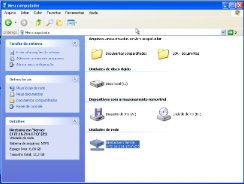
\includegraphics{figuras/mapeamento}}
   	\caption{Tela de um mapeamento}
    \label{mapeamento}
\end{figure} 

\pagebreak

\section{Compartilhamento de Impressoras}

O compartilhamento de impressora é a publicação das impressoras instaladas no servidor para que outras máquinas que estão na rede possam acessar e imprimir sem precisar da conexão local na impressora.

Para compartilhar as impressoras com o Samba 3 deve-se adicionar na seção [global] as variáveis contidas no Quadro \ref{smb_print}\\

\begin{lstlisting}[caption=Variáveis para permitir impressão em impressoras compartilhadas,label={smb_print}]	
[global]

printing = cups

load printers = yes	
\end{lstlisting}

\begin{itemize}
	\item \textbf{printing} - Define qual o programa será utilizado para gerenciar as impressões 
	\item \textbf{load printers} - Carrega as impressoras
\end{itemize}

O Samba 3 utiliza o cups que é o gerenciador de impressoras mais comum para o linux.

\begin{enumerate}
	\item \textbf{\#smbd -b $|$ grep CUPS} - Para saber se o pacote Samba 3 instalado é compatível com o CUPS. A saída deve ser algo como ``HAVE CUPS"
\end{enumerate}

Caso o cups não esteja instalado.

\begin{enumerate}
	\item \textbf{\#apt-get install cups} - Instala todos os pacotes necessários para o funcionamento do cups.
	\item \textbf{\$ firefox localhost:631} - Interface gráfica para gerenciar as impressoras. Figura \ref{cups}.
	\item \textbf{\# /etc/init.d/cupsys restart} - Reinicia o serviço do cups
\end{enumerate}

\begin{figure}[ht]
   	\centering
    \scalebox{1}{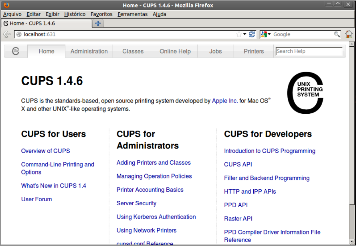
\includegraphics{figuras/cups}}
   	\caption{Tela do CUPS pelo Browser}
    \label{cups}
\end{figure}

Para habilitando o compartilhamento de impressora. Tem que adicionar as variáveis contidas no Quadro \ref{smb_printer}\\

\begin{lstlisting}[caption=Variáveis para compartilhar impressoras,label={smb_printer}]	
[printers]

print ok = yes

guest ok = yes

path = /var/spool/samba

browseable = yes	
\end{lstlisting}

\begin{itemize}
	\item \textbf{path} - Esse caminho é onde ficarão os spools de impressão. Esse diretório é criado automaticamente pelo Samba 3 e deve ter a permissão 777.
	\begin{enumerate}
		\item \textbf{chmod 777 -R /var/spool/samba}
	\end{enumerate}
\end{itemize}

Dessa forma ao acessar o servidor irão aparecer todas as impressoras instaladas.

\section{Instalação automática dos driver da impressora}

Para conectar-se a uma impressora compartilhada é necessário a instalação dos drivers da mesma. 

Um problema é como esses drivers são armazenados e instalados, já que uma das formas de instalar esses drivers é ir até o computador com o instalador em cd ou pen-drive e realizar a instalação manualmente, porém em uma grande rede se perde muito tempo com a locomoção e instalação. A solução desse problema é a instalação automática dos drivers, e com a utilização do Samba 3 os drivers serão instalados assim que o usuário tentar conectar a impressora.

Adiciona no [global]

\begin{itemize}
	\item \textbf{enable privileges = yes} - Permite privilégios a usuários
\end{itemize}

Criar um compartilhamento não visível onde ficará os drivers das impressoras. Conforme mostrado no Quadro \ref{smb_print_driver}\\

\begin{lstlisting}[caption=Variáveis para compartilhamento onde deverão ficar os \textit{drivers} das impressoras,label={smb_print_driver}]	
[print$]

path = /var/lib/samba/printers

read only = yes

write list = root

inherit permissions = yes	
\end{lstlisting}

\begin{itemize}
	\item \textbf{path} - Local onde os drivers serão instalados
	\item \textbf{write list} - Usuários ou grupos que terão permissão de escrita
	\item \textbf{inherit permissions} - Se os arquivos irão herdar as permissões da pasta.
\end{itemize}

Se o caminho apontado pelo path não existir ele terá que ser criado com as permissões necessárias.

\begin{enumerate}
	\item \textbf{\# mkdir -p /var/lib/samba/printers}
	
	\item \textbf{\# cd /var/lib/samba/printers}
	\item \textbf{\# mkdir WIN40 W32X86} - Essas pastas são os locais onde ficarão os drivers das impressoras, o WIN40 para sistemas Windows 95/98/ME e o W32X86 Windows NT/2000/XP.
	\item \textbf{\# chmod 2775 WIN40 W32X86} - Permissões especiais para instalar os drivers nos usuários.
	\item \textbf{\# net -S localhost -U root -W NOME\_DO\_SERVIDOR  rpc rights grant ``NOME DO SERVIDOR$\backslash$root" SePrintOperatorPrivilege} - Irá definir que o usuário root terá todas os privilégios necessários para gerenciar as impressoras.
\end{enumerate}

Com as permissões, usuários e impressoras configuradas, os \textit{drivers} tem que ser passados para o servidor. Para tal, é necessária a utilização de uma máquina cliente com Windows instalado. Ela se conectará ao servidor que está compartilhando as impressoras, e através da senha de root desse servidor, irá passar os \textit{drivers} através da rede. A sequência de figuras a seguir ilustra o passo-a-passo para a adição desses \textit{drivers}.

\begin{enumerate}
	\item \textbf{Acesse a maquina com um usuário local} - Figura \ref{login_windows_local}
		\begin{figure}[ht]
		   	\centering
		    \scalebox{1}{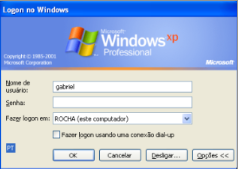
\includegraphics{figuras/login_windows_local}}
		   	\caption{Tela do Login no Windows localmente}
		    \label{login_windows_local}
		\end{figure}
		
	\item \textbf{Informe o endereço do servidor} - Figura \ref{server_ip}	
	\begin{figure}[ht]
	   	\centering
	    \scalebox{1}{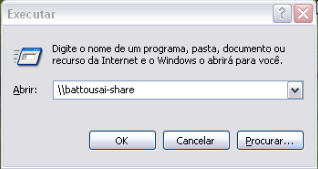
\includegraphics{figuras/server_ip}}
	   	\caption{IP do servidor de compartilhamento}
	    \label{server_ip}
	\end{figure}
		
\pagebreak
	
	\item \textbf{Informe o usuario root e sua senha.}	
	
	\item \textbf{Acesse a pasta ``Impressoras e aparelhos de fax"} - Figura \ref{impressora_aparelho_fax}
	\begin{figure}[ht]
	   	\centering
	    \scalebox{1}{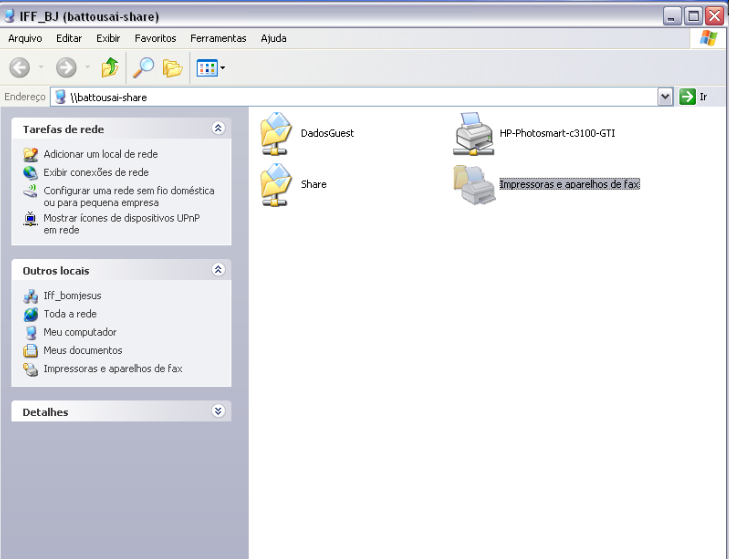
\includegraphics{figuras/impressora_aparelho_fax}}
	   	\caption{Impressoras e aparelhos de fax compartilhados}
	    \label{impressora_aparelho_fax}
	\end{figure}

%	\pagebreak

	\item \textbf{Clique na opção Arquivos -$>$ Propriedade do servidor.}
	
%	\pagebreak
	
 	\item \textbf{Aba Driver -$>$ Adicionar} - Figura \ref{adicionar_driver}
	\begin{figure}[ht]
	   	\centering
	    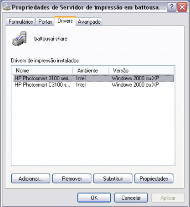
\includegraphics[width=0.5 \textwidth]{figuras/adicionar_driver}
	   	\caption{Adicionar driver ao servidor de impressão}
	    \label{adicionar_driver}
	\end{figure}
	
	\pagebreak
	
	\item \textbf{Selecione o driver da impressora que deve ser copiado para o servidor} - Figura \ref{selecionar_driver}
	\begin{figure}[ht]
	   	\centering
	    \scalebox{1}{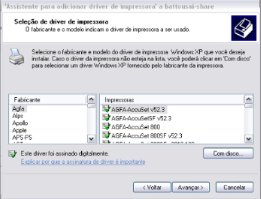
\includegraphics{figuras/selecionar_driver}}
	   	\caption{Selecionar o driver que será copiado para o servidor de impressão}
	    \label{selecionar_driver}
	\end{figure}
	
	
	\item \textbf{Selecione os sistemas operacionais dos \textit{drivers} que serão instalados, e avance até concluir o assistente.} - Figura \ref{selecionar_so}
	\begin{figure}[ht]
	   	\centering
	    \scalebox{1}{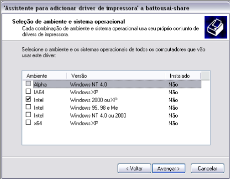
\includegraphics{figuras/selecionar_so}}
	   	\caption{Selecionar os Sistemas Operacional que o driver será compatível}
	    \label{selecionar_so}
	\end{figure}
	
	\pagebreak
	
	\item \textbf{Ao sair do assistente, clique com o botão direito na impressora desejada, e clique em Propriedades.} - Figura \ref{propriedade_impressora}
	\begin{figure}[ht]
	   	\centering
	    \scalebox{1}{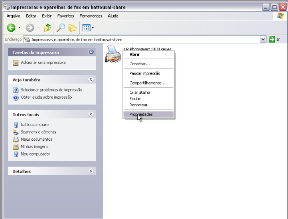
\includegraphics{figuras/propriedade_impressora}}
	   	\caption{Propriedade da impressora do compartilhamento}
	    \label{propriedade_impressora}
	\end{figure}

	
	\item \textbf{Na caixa de mensagem que irá aparecer, selecione a opção ``NÃO", pois caso selecione o sim o \textit{driver} será instalado somente na maquina local.} - Figura \ref{opcao_nao}
	\begin{figure}[ht]
	   	\centering
	    \scalebox{1}{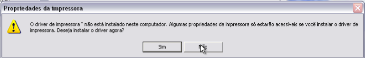
\includegraphics{figuras/opcao_nao}}
	   	\caption{Opção para não instalar o driver naquele momento}
	    \label{opcao_nao}
	\end{figure}
	
	\item \textbf{Na guia avançado, selecione o \textit{drive} que será vinculado a impressora e clique em OK.} - Figura \ref{aba_avancado}
	\begin{figure}[ht]
	   	\centering
	    \scalebox{1}{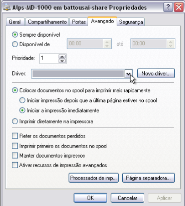
\includegraphics{figuras/aba_avancado}}
	   	\caption{Aba onde será feito o link da impressora com o driver}
	    \label{aba_avancado}
	\end{figure}
	
		\pagebreak
		
	\item \textbf{Após esses passos, o \textit{driver} da impressora já estará instalado no servidor de impressão. A partir desse momento, para instalar essa impressora, basta logar com o usuário do domínio no qual a impressora está compartilhada.} - Figura \ref{login_dominio}
	\begin{figure}[ht]
	   	\centering
	    \scalebox{1}{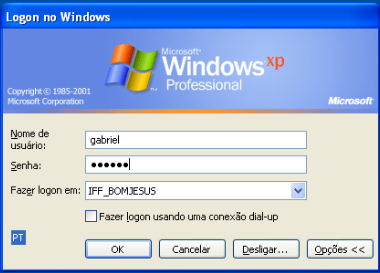
\includegraphics{figuras/login_dominio}}
	   	\caption{Logar no domínio}
	    \label{login_dominio}
	\end{figure}
	
	% \pagebreak
	
	\item \textbf{Acesse o servidor, conforme passo 2, e selecione a impressora que deseja mapear.} - Figura \ref{selecionar_impressora_servidor}
	\begin{figure}[ht]
	   	\centering
	    \scalebox{1}{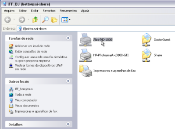
\includegraphics{figuras/selecionar_impressora_servidor}}
	   	\caption{Selecionar a impressora que será mapeado no usuário logado}
	    \label{selecionar_impressora_servidor}
	\end{figure}
	
%	\pagebreak
	
	\item \textbf{Após esses passos, a impressora será instalada automaticamente no computador cliente sem a necessidade de \textit{drivers} adicionais, pois estes foram disponibilizados automaticamente pelo servidor através da rede.} - Figura \ref{impressora_compartilhada}
	\begin{figure}[ht]
	   	\centering
	    \scalebox{1}{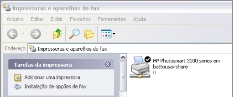
\includegraphics{figuras/impressora_compartilhada}}
	   	\caption{Impressora instalada no usuário}
	    \label{impressora_compartilhada}
	\end{figure}
	
\end{enumerate}

%\pagebreak

\section{Ingressando o Windows XP no Domínio}

Para ingressar um computador Windows no domínio através do Samba 3 é necessário que primeiramente ele esteja devidamente cadastrado no servidor Samba 3. O windows deve estar com os drivers de rede instalados e respondendo na rede.
Para ingressar o Windows XP no domínio deve-se realizar os seguintes passos:

\begin{enumerate}
	\item {Realize logon no windows com uma conta que possua privilégios administrativos. - Figura \ref{logon_local_adm}}
	\begin{figure}[ht]
   			\centering
   		 \scalebox{1}{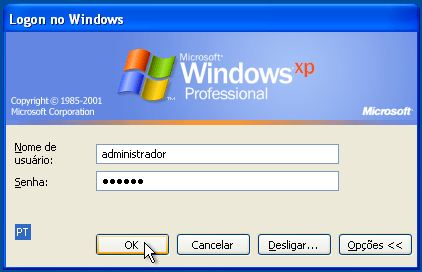
\includegraphics{figuras/logon_local_adm}}
   			\caption{Tela de logon local}
    		\label{logon_local_adm}
	\end{figure}

	\item {Após o logon, deve-se abrir o programa Executar no menu Iniciar e acessar as Propriedades do Sistema através do comando ``sysdm.cpl".}

	\item {Acessar a aba ``Nome do Computador". Deve-se clicar no botão ``Alterar". - Figura \ref{alterar_nome_micro}}

		\begin{figure}[ht]
	   			\centering
	   		 \scalebox{1}{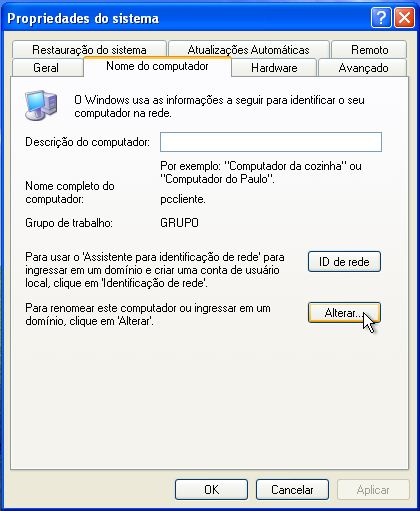
\includegraphics{figuras/alterar_nome_micro}}
	   			\caption{Alterando nome do micro}
	    		\label{alterar_nome_micro}
		\end{figure}
		 
		\pagebreak 

	\item {No menu de ``Alterações de nome do computador", certifique-se de que o nome definido para o computador é o mesmo que foi cadastrado no servidor Samba 3. No campo ``Membro de", selecione a opção ``Domínio" e digite o nome do domínio definido na sessão [global] do Samba 3 e depois clique em OK. - Figura \ref{incluir_dominio}} 
			\begin{figure}[ht]
		   			\centering
		   		 \scalebox{1}{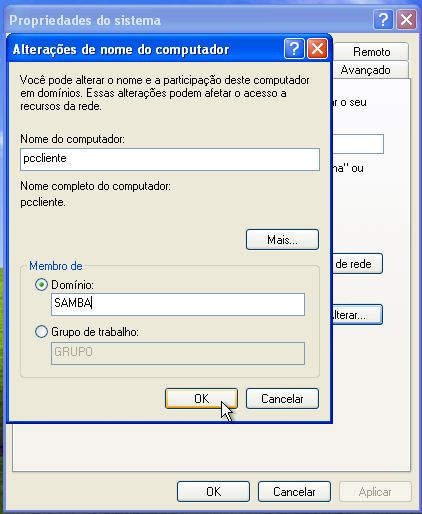
\includegraphics{figuras/incluir_dominio}}
		   			\caption{Incluir micro no domínio}
		    		\label{incluir_dominio}
			\end{figure}
	 
	%\pagebreak
	
	\item {Insira a senha de administrador do servidor para o micro ingressar no domínio. E aguarde a mensagem de confirmação.} 
	
	\item {Reinicie o micro quando for solicitado pelo sistema.}

	\item {Após inicialização o micro, selecione o domínio para realizar o logon e entre com um usuário e senha que esteja cadastrados previamente no servidor. - Figura \ref{logon}}
	\begin{figure}[ht]
			\centering
	 		\scalebox{1}{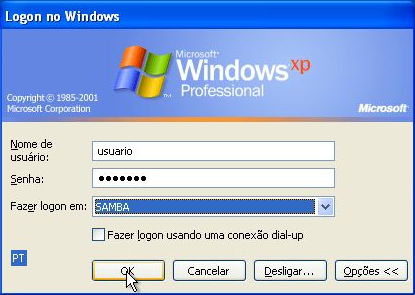
\includegraphics{figuras/logon}}
			\caption{Efetuando logon no domínio}
			\label{logon}
	\end{figure}

\end{enumerate}

%\pagebreak

\section{Ingressando o Linux no Domínio}

Para ingressar um computador linux no domínio é necessário que primeiramente ele esteja devidamente cadastrado no servidor Samba 3. Para o linux realize login no servidor PDC é necessário a instalação de três pacotes essenciais. São eles o Samba, o Winbind e os módulos do PAM (libpam-modules).

A instalação desses pacotes na distribuição Ubuntu pode ser realizada através dos comando:

\begin{enumerate}
	\item \textbf{\#apt-get update} - Atualiza a base de dados do repositório.
	\item \textbf{\#apt-get install samba winbind libpam-modules} - Realiza a instalação dos pacotes Samba, Winbind e módulos do PAM.
\end{enumerate}

Após a instalação é necessário realizar a configuração do micro para que possa fazer login no domínio. Começando pela configuração do Samba através do arquivo de configuração \textbf{/etc/samba/smb.conf}, que deve ser editado para que a seção [global] fique conforme o exemplo. Pode-se optar por adicionar essa configuração à configuração existente, ou pode manter apenas essa configuração básica:\\

\begin{lstlisting}[caption=FAZER,label={global}]	
[global]

workgroup = Dominio

netbios name = cliente1

winbind use default domain = yes

obey pam restrictions = yes

security = domain

encrypt passwords = true

wins server = 192.168.1.1

winbind uid = 10000-20000

winbind gid = 10000-20000

template shell = /bin/bash

template homedir = /home/\%U
\end{lstlisting}

Explicação de algumas variáveis importantes:
\begin{itemize}
	\item \textbf{workgroup} - Nome do domínio configurado no servidor Samba 3.
	\item \textbf{netbios name} - Nome do computador cliente (/etc/hostname), que deve estar cadastrado no servidor.
	\item \textbf{wins server} - Ip do servidor PDC Samba 3.
\end{itemize}

Editado o arquivo \textbf{/etc/samba/smb.conf}, deve-se testar o arquivo de configuração para verificação de erros através do comando \textbf{\#testparm}.
Após a configuração do Samba, deve-se configurar o arquivo \textit{Network Services Switch} (\textbf{/etc/nsswitch.conf}), que determina a ordem das buscas quando uma informação é solicitada. Esse arquivo deve ter as seguintes linhas alteradas:\\

\begin{lstlisting}[caption=FAZER,label={global}]	
passwd: compat winbind

group: compat winbind

shadow: compat winbind	
\end{lstlisting}

Foi incluído o \textbf{winbind} nas variáveis de busca \textbf{passwd}, \textbf{group} e \textbf{shadow} para que esses valores sejam buscados no servidor Samba 3.

Depois de concluídas as configurações, é necessário reiniciar o Samba e o Winbind.

\begin{enumerate}
	\item \#service winbind restart
	\item \#service smbd restart
	\item \#service nmbd restart	
\end{enumerate}


Para testar a configuração realizada deve-se fazer o ingresso no domínio conforme abaixo. Será retornada uma mensagem de sucesso.\\

\begin{itemize}
	\item \#net rpc join member -U root
\end{itemize}

\begin{lstlisting}[caption=FAZER,label={global}]	
Password:

Joined domain DOMINIO.
\end{lstlisting}

A senha solicitada é a senha de root do servidor PDC, cadastrada no Samba.

Os arquivos a serem alterados em seguida serão as os arquivos de políticas de funcionamento do PAM. Essas políticas se encontram no diretório \textbf{/etc/pam.d}, onde está contido os arquivos de configuração pra cada serviço que utilize os módulos de autenticação do PAM. O nome de um arquivo nesse diretório indica a qual serviço o arquivo de configuração se refere (portanto o arquivo \textbf{/etc/pam.d/login} fará referência ao serviço de \textit{LOGIN} do Linux).
Para definir políticas de autenticação a um serviço, deve-se acessar o arquivo do serviço desejado acrescentar as configurações desejadas seguindo a seguinte sintaxe:\\

\begin{lstlisting}[caption=FAZER,label={global}]	
auth	required	pam_nologin.so	no_warn
\end{lstlisting}

Cada linha de configuração é formada por 4 campos. No exemplo temos os 4 campos na seguinte ordem: Nome instalação, tag de controle, nome do módulo, e argumentos do módulo. Campos adicionais serão interpretados como argumentos do módulo.

Após o teste de ingresso no domínio é necessário configurar o sistema de autenticação PAM para busca os logins no servidor. Para isso é necessário modificar os arquivos \textbf{/etc/pam.d/login} e \textbf{/etc/pam.d/gdm}. O arquivo \textbf{/etc/pam.d/login} é responsável pelas configurações de autenticação de usuários no sistema, enquanto o arquivo \textbf{/etc/pam.d/gdm} é responsável pelas configurações de autenticação na interface de login do gnome.
No arquivo \textbf{/etc/pam.d/login}, deve-se adicionar as linhas abaixo ao inicio do arquivo:\\

\begin{lstlisting}[caption=FAZER,label={global}]
session required pam_mkhomedir.so skel=/etc/skel umask=0022

session optional pam_mount.so

auth sufficient pam_winbind.so

account sufficient pam_winbind.so

session required pam_winbind.so
\end{lstlisting}

No arquivo \textbf{/etc/pam.d/gdm} deve-se comentar todo o seu conteúdo e adicionar as linhas abaixo ao inicio do arquivo:\\

\pagebreak

\begin{lstlisting}[caption=FAZER,label={global}]	
auth required /lib/security/pam_securetty.so

auth required /lib/security/pam_nologin.so

auth sufficient /lib/security/pam_winbind.so

auth required /lib/security/pam_pwdb.so use_first_pass shadow nullok

account required /lib/security/pam_winbind.so

session required /lib/security/pam_mkhomedir.so skel=/etc/skel umask=0022
\end{lstlisting}

As configurações acima fazem o GDM exibir uma os usuários disponíveis no servidor para login diretamente no domínio sem que haja autenticação local. Para as configurações acima funcionarem corretamente, a opção de Login Automático não pode estar ativada no computador. % Cria o capítulo 3
\chapter{SAMBA 4}

O samba 4 vem com a proposta de criar um Active Directory livre, utilizando o LDAP, Bind e Kerberos.

\section{Instalação do SAMBA4}

Antes de começar a instalação o relógio do servidor tem que estar atualizado.

\begin{itemize}
	\item \textbf{\# ntpdate br.pool.ntp.org} - Atualiza a hora do servidor a partir do servidor br.pool.ntp.org.
\end{itemize}

Por se tratar de um sistema ainda em fase de produção alguns erros podem aparecer ou alguns parâmetros devem ser modificados.

\begin{itemize}
	\item \textbf{\# apt-get install build-essential libattr1-dev libblkid-dev libgnutls-dev python-dev autoconf python-dnspython git-core} - Pacotes necessários para a compilação do samba 4 e download;
	\item \textbf{\# git clone git://git.samba.org/samba.git samba-master; cd samba-master} - Faz um clone do samba 4 que esta no repositório para o servidor;
	\item \textbf{\# ./configure.developer} - Configurar as bibliotecas com parâmetros de desenvolvedor. Habilitando alguns modos de debug;
	\item \textbf{\# make} - Faz uma leitura do comando Makefile;
	\item \textbf{\# make install} - Executa os comandos configurados para o parâmetro install do arquivo Makefile;
	\item \textbf{\# /usr/local/samba/sbin/provision - -use-ntvfs - -realm=iff.bomjesus - -domain=iff  - -adminpass= Senha00 - -server-role='domain controller'} - Cria o domínio samba com AD;
		\begin{enumerate}
			\item \textbf{use-ntvfs} - Habilita o NTVFS;
			\item \textbf{realm} - Domínio do servidor Kerberos;
			\item \textbf{domain} - Domínio do samba;
			\item \textbf{adminpass} - Senha do Administrator, essa senha deve ter pelo menos uma letra maiúscula;
			\item \textbf{server-role} - Regra do servidor.
		\end{enumerate}
	\item \textbf{\# /usr/local/samba/bin/smbclient --version} - Mostra a versão do samba;
	\item \textbf{\# /usr/local/samba/sbin/samba -i -M single} - Inicia o samba 4 com o modo debug;
	\item \textbf{\#  echo 'ip do servidor iff.bomjesus iff' $>$$>$ /etc/hosts} - Define um nome para o ip do servidor.
\end{itemize}

\section{Instalação e configuração do BIND9}

O samba 4 já vem pré configurado para trabalhar com BIND9 para ser o servidor DNS.

\begin{itemize}
	\item \textbf{\# wget ftp://ftp.isc.org/isc/bind9/9.9.0/bind-9.9.0.tar.gz} - Download da versão 9.9 do bind9;
	\item \textbf{\# tar xzvf bind-9.9.0.tar.gz} - Descompactar o pacote do bind9;
	\item \textbf{\# cd bind-9.9.0} - Acessar o diretório do bind9 descompactado;
	\item \textbf{\# ./configure --prefix=/usr/local/bind9 --sysconfdir=/etc/bind} - Configurar os parâmentros para a instalação do bind, tais como o local onde vai ser instalado e onde ficarão os arquivos de configuração;
	\item \textbf{\# make} - Leitura do comando Makefile;
	\item \textbf{\# make install} - Executa os comandos configurados para o parâmetro install do arquivo Makefile;
	\item \textbf{\# cd /etc/bind} - Acessar o diretório onde se encontram os arquivos do bind;
	\item \textbf{\# vim named.conf} - Cria e edita o arquivo. Adicione as linhas abaixo no arquivo;
		\begin{enumerate}
			\item \textbf{include "/etc/bind/named.conf.options";}
			\item \textbf{include "/etc/bind/named.conf.local";}
		\end{enumerate}
 		\item \textbf{\# vim named.conf.options}
			\begin{enumerate}
				\item \textbf{Adicionar no arquivo} - options \{
        			
					directory "/var/cache/bind";

					auth-nxdomain no;

					listen-on-v6 \{ any; \};
					
					\};
			\end{enumerate}
\end{itemize}

O comando provision gera os arquivos de configuração necessários para o funcionamento do samba com o servidor dns.

\begin{itemize}
	\item \textbf{\# vim named.conf.local} -  Adicione a linha abaixo no arquivo;
		\begin{enumerate}
			\item \textbf{include "/usr/local/samba/private/named.conf";}
		\end{enumerate}
\end{itemize}

Comentar as linhas conforme a versão do bind9 

\begin{itemize}
	\item \textbf{\# vim /usr/local/samba/private/named.conf}
\end{itemize}

\# For BIND 9.8.0

    \# database "dlopen /usr/local/samba/lib/bind9/dlz\_bind9.so"; 

Descomentar

 \# For BIND 9.9.0

    database "dlopen /usr/local/samba/lib/bind9/dlz\_bind9\_9.so";

\begin{itemize}
	\item \textbf{\# groupadd named \&\& useradd named -g named} - Cria o usuário responsável pelo bind e o insere no grupo named;
	\item \textbf{\# mkdir /var/cache/bind} - Cria a pasta onde ficarão os caches do bind;
	\item \textbf{\# /usr/local/bind9/sbin/named -u named -g} - Inicia o bind com o usuário named;
\end{itemize}

O servidor samba tem que ter seu endereço DNS configurado para apontar para seu servidor DNS.

\begin{itemize}
	\item \textbf{\# echo 'nameserver "ip do servidor"' $>$$>$ /etc/resolv.conf} - Define o endereço do servidor de DNS que o computador irá enviar suas solicitações;
\end{itemize}

A partir de agora para acessar a internet através do servidor samba o bind deverá estar sendo executado.

\section{Instalação do Kerberos}

O kerberos a ser instalado é o Heimdal

\begin{itemize}
	\item \textbf{\# apt-get install krb5-user krb5-kdc krb5-config kstart} - Instala todos os pacotes necessários e faz as referências necessárias.
\end{itemize}

Após instalar os pacotes, substitua o /etc/krb5.conf pelo arquivo criado e pré-configurado pelo samba que esta localizado em /usr/local/samba/private/krb5.conf

\begin{itemize}
	\item \textbf{\# cp /usr/local/samba/private/krb5.conf  /etc/}
\end{itemize}

Teste para verificar se todos as configurações foram realizadas corretamente

\begin{itemize}
	\item \textbf{\# host -t SRV \_ldap.\_tcp.iff.bomjesus.} - O resultado deve ser parecido : \textbf{\_ldap.\_tcp.iff. bomjesus has SRV record 0 100 389 server.iff.bomjesus.}
	\item \textbf{\# host -t SRV \_kerberos.\_udp. iff.bomjesus.} - O resultado deve ser parecido : \textbf{\_kerberos. \_udp.iff.bomjesus has SRV record 0 100 88 server.iff.bomjesus.}
	\item \textbf{\# host -t A iff.bomjesus} - O resultado deve ser parecido : \textbf{iff.bomjesus has address 172.16.214.167}
\end{itemize}

\section{Kerberos com Bind9}

Configurar atualizações dinâmicas no DNS com o kerberos

Para o funcionamento das atualizações algumas variáveis necessárias de sistema devem ser criadas para o acesso do kerberos com bind

\begin{itemize}
	\item \textbf{\# KEYTAB\_FILE="/usr/local/samba/private/dns.keytab"}
	\item \textbf{\# KRB5\_KTNAME="/usr/local/samba/private/dns.keytab"}
	\item \textbf{\# export KEYTAB\_FILE}
	\item \textbf{\# export KRB5\_KTNAME}
\end{itemize}

Mudar o dono e o grupo do dns.keytab para que o bind possa alterar o arquivo

\begin{itemize}
	\item \textbf{\# chown named:named /usr/local/samba/private/dns.keytab}
	\item \textbf{\# /usr/local/samba/sbin/samba\_dnsupdate --verbose}
\end{itemize}

\section{AD}

Pacotes necessários para gerenciar o AD no linux XP ou windows server.

\section{GPO}

Pacotes necessários para gerenciar as GPO's no linux XP ou windows server.

\section{Compartilhamento de arquivos e impressoras}

SAMBA4 ainda não consegue compartilhar arquivos e impressoras, e tem problemas com a integração dos usuários e grupos do Active Directory com os locais, dificultando a definição das permissões a arquivos e diretórios.

Uma solução para tal problema é identificar o código do usuário no Active Directory e dar as devidas permissões a pasta desejada.

\begin{itemize}
	\item \textbf{/usr/local/samba/bin/wbinfo --name-to-sid USERNAME} - O resultado deve ser o sid do usuário no samba. ex: S-1-5-21-4036476082-4153129556-3089177936-1005 SID_USER (1)
	\item \textbf{bin/wbinfo --sid-to-uid S-1-5-21-4036476082-4153129556-3089177936-1005} - Mostra o id do usuário e é a referência do usuário local com o do samba 4.
	\item \textbf{chown 3000011 /home/usuario/} - Mudando o usuário do diretório e as suas permissões, o usuário do AD irá ter o acesso aos arquivos.
\end{itemize} 

\section{Perfil Móvel}

Muito parecido com o samba3 criar um compartilhamento no samba e dar as devidas permissões a pasta. A diferença se da na hora de definir que será perfil movel.

***FIGURA DO AD DEFININDO PERFIL MOVEL***

\section{Gerenciando o Samba4}

O samba-tools - Gerência o samba. Com ele se poder criar usuários, grupos, gpo's e outras funções do Active Directory, porém um forma de texto.

***FIGURA DO SAMBA-TOOLS***

\section{Samba3 no AD Samba4}

\section{Script para adicionar maquina linux no AD}

\section{Windows no domínio Samba 4} % Cria o capítulo 4
\chapter{ESTUDO DE CASO}

Esta proposta de implementação foi motivada através de um cenário de instituição de ensino que necessitava de uma otimização na segurança e compartilhamento de seus recursos de TI. Para melhor gerenciamento e manutenção dos arquivos compartilhados e usuários na rede, seria necessária a implantação de um servidor que centralizasse todas essas tarefas.
Após identificada a necessidade desse novo recurso, foi iniciada uma pesquisa para encontrar um software que atendesse os requisitos. O Windows Server em todas as suas versões até hoje lançadas poderia ser a solução, mas é proprietário e o valor de uma licença da versão 2012 \textit{Datacenter} custa, atualmente, em torno de 10 mil reais \ref{SERVER}. O alto valor da licença acaba inviabilizando a utilização da mesma nas instituições  de ensino e em pequenas empresas. 
Para solucionar esse problema da compra de licenças foi criada uma versão livre, o Samba 4, que faz as mesmas tarefas de um Windows Server, trabalhando com o mesmo protocolo, o LDAP. Por ser livre, foi utilizada neste trabalho.
A instituição abordada neste trabalho contém 110 computadores nos setores administrativos e 90 nos laboratórios de informática. Abaixo uma pequena demonstração da estrutura da rede:

\begin{figure}[ht]
   	\centering
    \scalebox{1}{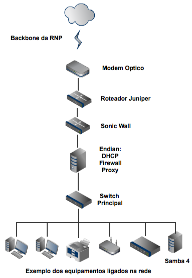
\includegraphics{figuras/iff}}
   	\caption{Estrutura da rede do instituto}
    \label{rede}
\end{figure}
          				
Os setores são divididos conforme suas funções no organograma da instituição. Os principais são:

* Diretoria do Departamento de Administração e Finanças

* Diretoria do Departamento de Gestão de Pessoas

* Coordenação de Registros Acadêmicos

* Chefe de Gabinete

Com a proposta de implementação abordada neste trabalho, cada setor e usuário terá na rede um compartilhamento próprio, com suas permissões definidas. Dois servidor serão inseridos na rede com as seguintes configurações:

\begin{itemize}
	\item{Processador Intel Core I7\textregistered}
	\item{4GB de memória RAM}
	\item{Um servidor com 6 Tb de HD e o outro com 100 Gb de HD}
	\item{Placas de vídeo, áudio e rede Onboard}
\end{itemize}

Em ambos os servidores foi instalado o sistema operacional Debian 6.0.5. Por trabalharem com o mesmo protocolo e para não ocorrer conflitos, o Samba 3 foi instalado em máquina diferente do Samba 4. Sendo assim ficaram as maquinas:

\begin{itemize}
	\item{Servidor de 6TB com sistema operacional Debian 6.0.5 e Samba 3}
	\item{Servidor de 100Gb com sistema operacional Debian 6.0.5 e Samba 4}
\end{itemize}

Antes da instalação do Samba 4 seus pré requisitos foram instalados e configurados como o DNS Bind 9.9 e o Kerberos Heimdal com suas variáveis de ambiente.
Após a configuração dos sistemas básicos, o Samba 4 foi configurado com os seguintes parâmetros.

\# cd /usr/local/samba/

\# sbin/provision "--use-ntvfs "--realm=instituto.ensino "--domain=instituto "--adminpass= Senha12 "--server-role=’domain controller’

Com o samba 4 já configurado e com as modificações no named.conf.local do bind realizadas, foi inserido no domínio do active directory  as máquinas Windows XP e as máquinas Linux, através do script smbad.sh, que se encontram na rede.

Por não ter uma ferramenta mais completa para o gerenciamento do Samba 4 pelo Linux, um computador com Windows XP foi designado para tal tarefa. Nele foram instalados o adminpack e o gerenciador de gpo do Windows. Por trabalharem com o mesmo protocolo como já foi dito anteriormente não houveram incompatibilidades na utilização das ferramentas.

Os usuários foram criados a partir da interface gráfica do adminpack no Windows, respeitando os requisitos de nome completo, ramal da sala, sala, entre outras informações que auxiliam na identificação dos usuários no AD e inseridos nos respectivos grupos dos seus setores.

Com os usuários cadastrados e inseridos em seus grupos, foram criadas as GPO`s com os scripts de inicialização e nelas foram definidos os mapeamentos automáticos dos compartilhamentos

O servidor que contém o Samba 3 foi inserido no Active Directory pelo scritpt smbad.sh. Com o servidor logando através do AD, as regras de segurança e permissões dos usuários criadas no Samba 3 irão valer para os usuários contidos no AD. Foram criados compartilhamentos com os nomes dos setores mais importantes da instituição afim de melhorar e garantir o melhor trabalhos das pessoas no setor.

Seções inseridas no smb.conf

Obs:  As seções foram inseridas com a sigla dos setores e os valores da seção global são alterados pelo script smbad.sh

[Chefia\_de\_Gabinete]

comment = Chefia de gabinete

path = /srv/samba/chefia

valid users = +direcao

read only = no

force group = direcao

browseable = no

veto files = *.wmv/*.avi/*.wma/*.mp?/*.flv

[DDAF] 

comment = Diretoria do Departamento de Administração e Finanças

path = /srv/samba/ddaf

valid users = +ddaf

read only = no

force group = ddaf

browseable = no

veto files = *.wmv/*.avi/*.wma/*.mp?/*.flv

[DDGP] 

comment = Diretoria do Departamento de Gestão de Pessoas

path = /srv/samba/ddgp

valid users = +ddgp

read only = no

force group = ddgp

browseable = no

veto files = *.wmv/*.avi/*.wma/*.mp?/*.flv

[CRA] 

comment = Coordenação de Registros Acadêmicos

path = /srv/samba/cra

valid users = +registro

read only = no

force group = registro

browseable = no

veto files = *.wmv/*.avi/*.wma/*.mp?/*.flv


[HOME] 

comment = Pasta dos usuários

path = /srv/samba/\%U

valid users = \%U

read only = no

browseable = no

veto files = *.wmv/*.avi/*.wma/*.mp?/*.flv

Com as sessões criadas no samba, as pastas foram criadas no /srv e atribuídas as permissões 770 com o proprietário root e o grupo com o nome do setor ou do usuário que será designado a pasta:

mkdir /srv/samba/ddgp

chmod 770 -R /srv/samba/ddgp

chown root:ddgp -R /srv/samba/ddgp

Todas as impressoras foram colocadas na rede, mapeadas no servidor do Samba 3 e compartilhadas para os demais computadores com a instalação dos drives automática.

[printers] 

print ok = yes 

guest ok = yes

path = /var/spool/samba 

browseable = yes

[print\$] 

path = /var/lib/samba/printers 

read only = yes

write list = root 

inherit permissions = yes

%\section{Objetivos alcançados}
%\section{Trabalhos futuros} % Cria o capítulo 5
\chapter{CONCLUSÕES}

Neste trabalho foi apresentada uma proposta de implantação de um servidor de modo a melhorar o acesso dos usuários da instituto aos recursos de autenticação dos usuários, compartilhamento de arquivos e compartilhamento de impressoras na rede e ainda assegurar a disponibilidade dos mesmos, independente do equipamento utilizado. Antes da implantação dos servidores todos os serviços eram atrelados à máquina local do usuário assim impedindo que o usuário a usasse em outra máquinas da rede.

Além disso, foi possível mostrar que, ao realizar esta implantação, o administrador de rede terá um maior controle dos acessos dos usuários já que a conta do usuário não fica mais atrelada uma única máquina e o Samba 4 oferece uma opção de visualizar todos os usuários cadastrados e podendo permitir ou negar recursos, por exemplo.

Foi possível ainda discutir sobre ferramentas disponíveis para a realização da implantação da proposta, de forma simples e objetiva, focada na estrutura abordada para receber o servidor, além de configurações e \textit{scripts} criados para auxiliar o processo.

O Samba 4 funcionou perfeitamente no que se propõe a fazer, mesmo sendo uma versão \textit{Release Candidate} e com o lançamento de uma versão estável Samba 4 irá tornar o Samba 3 desnecessário.

Como em qualquer trabalho que envolve ferramentas em evolução, neste trabalho serão necessárias melhorias e novas pesquisas, não permitindo que o mesmo fique ultrapassado e não seja compatível com as ferramentas em constante atualização.

Após o lançamento da versão estável do Samba 4 poderá ser feita uma nova pesquisa para a análise de comportamento e se ela pode ser aplicada em grande empresas e com um grande número de usuários.



 % Cria o capítulo 6
\bibliography{referencia} % Gera as referências bibliográficas
\appendix 

\chapter{Scripts}

\section{smbda.sh}
%Apêndices são opcionais, mas podem ser usados, por exemplo, para incluir tabelas com os dados brutos.

\#!/bin/sh
 
\#\#\#\#\#\#\#\#\#\#\#\#\#\#\#\#\#\#\#\#\#\#\#\#\#\#\#\#\#\#\#\#\#\#\#\#\#\#\#\#\#\#\#\#\#\#\#\#\#\#\#\#\#\#\#\#\#\#\#\#\#\#\#\#\#\#

\# Copyright (C) 2011 - Fabio Antonio Ferreira \hspace{160pt} \#

\# http://fantonio.wordpress.com | fantonios@gmail.com \hspace{106pt} \#

\# Este trabalho está licenciado sob uma Licença Creative Commons \hspace{59pt} \#

\# Atribuição-Compartilhamento pela mesma Licença 2.5 Brasil. Para ver a copia \#

\# desta licença, acesse: http://creativecommons.org/licenses/by-sa/2.5/br/ \hspace{34pt} \#

\# ou envie uma carta para Creative Commons, 171 Second Street, Suite 300, \hspace{19pt} \#

\# San Francisco, California 94105, USA. \hspace{188pt} \#

\# Modificações em 27 de Julho de 2012 por Gabriel Rocha (GBR) \hspace{67pt}             \#

\# email: gabriel.rocha.gbr@gmail.com \hspace{198pt} \#

\#\#\#\#\#\#\#\#\#\#\#\#\#\#\#\#\#\#\#\#\#\#\#\#\#\#\#\#\#\#\#\#\#\#\#\#\#\#\#\#\#\#\#\#\#\#\#\#\#\#\#\#\#\#\#\#\#\#\#\#\#\#\#\#\#\#

\# == FUNCOES ===============================================

USUARIO=`whoami`

if [ "\$USUARIO" != "root" ]; then

 	echo

  echo "======================================================"

  echo " ESTE PROGRAMA PRECISA SER EXECUTADO COM PERMISSOES DE SUPERUSUARIO!"  

  echo " Abortando..."

  echo "======================================================"

  echo

  exit 1

fi

\_HEAD () \{

`which clear`

echo "SISTEMA PARA ADICIONAR MAQUINA LINUX AO DOMÍNIO WINDOWS OU LINUX"

echo "========================================================="

\}

\_PACOTES () \{

        echo "Instalando os pacotes necessários";       


  apt-get install krb5-user libpam-krb5 winbind samba smbfs smbclient krb5-config libkrb53 libkdb5-4 libgssrpc4 -y $>$ /dev/null;
  
      check=\$(echo \$?)

        if [ \$check -eq 0 ]; then

           echo "Pacotes instalados com sucesso"

        else

           echo "Falha ao instalar os pacotes"

        fi

\}

\_HORA () \{

        echo "Atualizando data e hora";

        ntpdate br.pool.ntp.org $>$ /dev/null;

        echo "Horario atual:" `date`

        echo "Hora alterada com sucesso"

\}

\_BACKUP\_ORIG () \{

  \# Rotina de Backup dos arquivos de configurações.

	if [ ! -e /etc/krb5.conf\_backup ]; then

		cp /etc/krb5.conf /etc/krb5.conf\_backup $>$ /dev/null;

	fi

	if [ ! -e /etc/resolv.conf\_backup ]; then

		cp /etc/resolv.conf /etc/resolv.conf\_backup $>$ /dev/null

	fi

	if [ ! -e /etc/samba/smb.conf\_backup ]; then

        	cp /etc/samba/smb.conf /etc/samba/smb.conf\_backup $>$ /dev/null

	fi

	if [ ! -e /etc/nsswitch.conf\_backup ]; then

        	cp /etc/nsswitch.conf /etc/nsswitch.conf\_backup $>$ /dev/null

	fi

	if [ ! -e /etc/pam.d/common-account\_backup ]; then

	        cp /etc/pam.d/common-account /etc/pam.d/common-account\_backup $>$ /dev/null

	fi

	if [ ! -e /etc/pam.d/common-auth\_backup ]; then

	        cp /etc/pam.d/common-auth /etc/pam.d/common-auth\_backup $>$ /dev/null

	fi

	if [ ! -e /etc/pam.d/common-session\_backup ]; then

	        cp /etc/pam.d/common-session /etc/pam.d/common-session\_backup $>$ /dev/null

	fi

	if [ ! -e /etc/pam.d/sudo\_backup ]; then

	        cp /etc/pam.d/sudo /etc/pam.d/sudo\_backup $>$ /dev/null

	fi
         
        check=\$(echo \$?)

   if [ \$check -eq 0 ]; then

      echo "Rotina de Backup executada com sucesso!"

   else

      echo "Falha ao fazer o Backup."

   fi
         
\}

\_RETURN\_BACKUP () \{

        \# Rotina de Recuperação do Backup de configurações.

        mv /etc/krb5.conf\_backup /etc/krb5.conf $>$ /dev/null

        mv /etc/resolv.conf\_backup /etc/resolv.conf $>$ /dev/null

        mv /etc/samba/smb.conf\_backup /etc/samba/smb.conf $>$ /dev/null

        mv /etc/nsswitch.conf\_backup /etc/nsswitch.conf $>$ /dev/null

        mv /etc/pam.d/common-account\_backup /etc/pam.d/common-account $>$ /dev/null

        mv /etc/pam.d/common-auth\_backup /etc/pam.d/common-auth $>$ /dev/null
        
        mv /etc/pam.d/common-session\_backup /etc/pam.d/common-session $>$ /dev/null

        mv /etc/pam.d/sudo\_backup /etc/pam.d/sudo $>$ /dev/null
         
        
				check=\$(echo \$?)

   if [ \$check -eq 0 ]; then

      echo "Recuperação do Backup executada com sucesso!"

   else

      echo "Falha na recuperação do Backup."

   fi
         
\}

\_NOME\_DOMINIO () \{
 
   \#Entrada do nome do dominio ao qual deseja engreçar.

	 \#No caso do linux temos dois servidores um do KDC e outro do dominio

	 \#No windows informamos o servidor kdc

    read -p "Entre com o nome do Domínio:" var1

    dominio=\$(echo \$var1 | tr a-z A-Z)

    read -p "Entre com o seu KDC (key Distribution Center):" var2

    kdc=\$(echo \$var2 | tr A-Z a-z)         

\}

\_IP\_DNS (){

	\#IP do servidor de dns

	read -p "Entre com o IP do servidor de DNS:" ip

	echo "nameserver \$ip" $>$ /etc/resolv.conf

\}

\_SO\_SERVIDOR () \{

	\#Sistema Operacional do AD	

	read -p "Entre com o S.O. do servidor (Linux ou Windows): " so

	so=\$(echo \$so | tr a-z A-Z)

	workgroup=""

	if [ \$so = "LINUX" ] ; then

		read -p "Informe o Domain do Samba4: " workgroup

		workgroup=\$(echo \$workgroup | tr a-z A-Z)

	else

		workgroup=\$(echo \$var1)

	fi

\}

\_KRB5 () \{

   echo "[libdefaults]

   default\_realm = \$dominio

	 \# The following krb5.conf variables are only for MIT Kerberos.

      krb4\_config = /etc/krb.conf

      krb4\_realms = /etc/krb.realms

      kdc\_timesync = 1

      ccache\_type = 4

      forwardable = true

      proxiable = true

		\# The following libdefaults parameters are only for Heimdal Kerberos.

      v4\_instance\_resolve = false

      v4\_name\_convert = \{

           host = \{

               rcmd = host

               ftp = ftp

           \}  

           plain = \{

               something = something-else

           \}  

      \}  

      fcc-mit-ticketflags = true

   [realms]

   		\$dominio = \{

        	kdc = \$kdc
           
            admin\_server = \$kdc

           \}  
             
   [domain\_realm]

   		.\$var1 = \$kdc

   [login]

   		krb4\_convert = true

   		krb4\_get\_tickets = false" $>$ /etc/krb5.conf
 
   echo "Configuração alterada com sucesso!"

\}

\_TESTEAD () \{

   read -p "Entre com um usuário para testar sua conexão com o Active Directory:" user

   kinit \$user$@$\$dominio

    

   check=\$(echo \$?)

   if [ \$check -eq 0 ]; then

      echo "Sua máquina conectou com sucesso!"

   else

      echo "Falha ao se conectar com o Active Directory"

   fi

\}

\_SMB () \{

    

   maquina=\$(hostname)

   echo "\# Sample configuration file for the Samba suite for Debian GNU/Linux.

   \#======================= Global Settings =======================

   [global]

      workgroup = \$workgroup

      netbios name = \$maquina

      realm = \$var1

      server string = \% h Server

      dns proxy = no

  	  log file = /var/log/samba/log.\%m  

	  max log size = 1000

	  syslog = 0  

      panic action = /usr/share/samba/panic-action \%d

      security = ADS

      password server = \$kdc

      encrypt passwords = true

      passdb backend = tdbsam

      obey pam restrictions = yes

      unix password sync = yes

      passwd program = /usr/bin/passwd \%u
      
      pam password change = yes

      idmap uid = 10000-20000

      winbind gid = 10000-20000

      winbind enum users = yes

      winbind enum groups = yes

      winbind use default domain = yes

      template homedir = /home/\%D/\%U

      template shell = /bin/bash

   [homes]

      comment = Home Directories

      browseable = no

      read only = yes

      create mask = 0700

      directory mask = 0700

      valid users = \%S " $>$ /etc/samba/smb.conf

   echo "Configuração alterada com sucesso!"

\}

\_FUNC\_RESTART() \{

        \# Stop Winbind

        /etc/init.d/winbind stop $>$ /dev/null

        check=\$(echo \$?)

   if [ \$check -eq 0 ]; then

      echo "Winbind Stop!"

   else

      echo "Falha ao parar o Winbind"

   fi

     \# Restart Samba

     /etc/init.d/smbd restart $>$ /dev/null

     check=\$(echo \$?)

   if [ \$check -eq 0 ]; then

      echo "Samba restart com sucesso!"

   else

      echo "Falha no restart do Samba!"

   fi

    \# Start Winbind

    /etc/init.d/winbind start $>$ /dev/null

    check=\$(echo \$?)

   if [ \$check -eq 0 ]; then

      echo "Winbind start!"

   else

      echo "Falha ao fazer iniciar o Winbind!"

   fi

\}

\_ADDDOMINIO () \{
    
 
  echo "++++++++++++++++++++++++++++++++++++++++++++"

   echo "++  Adicionando a Máquina no Domínio  ++"

   echo "++++++++++++++++++++++++++++++++++++++++++++"

   \# Adicionando a máquina ao domínio

        read -p "Entre com um usuário administrador de Domínio:" user   

   net ads join -U \$user;

        check=\$(echo \$?)

        clear

        \# Validação da conexão com o domínio

        if [ \$check -eq 0 ]; then

      echo "Sua máquina foi adicionada no Domínio!"

   else

      echo "Falha ao adicionar a máquina no Domínio"

   fi

\}

\_TESTDOMINIO () \{

        \# Teste de requisição ao dominio

        wbinfo -t $>$ /dev/null

        check=\$(echo \$?)

   if [ \$check -eq 0 ]; then

      echo "Teste de Domínio!"

   else

      echo "Falha ao testar o Domínio"

   fi

\}

\_FUNCAUTENTICACAO () \{

        \# Configurando o arquivo nsswitch.conf

        echo "passwd:         compat winbind

              group:          compat winbind

              shadow:         compat" $>$ /etc/nsswitch.conf

        \# Teste de configuração do Winbind        

        check=\$(echo \$?)
   		
		if [ \$check -eq 0 ]; then

      echo "Winbind testado com sucesso!"

   else

      echo "Falha ao testar o Winbind"

   fi

        \# PAM - common-account

        echo "account sufficient       pam\_winbind.so
              account required         pam\_unix.so" $>$ /etc/pam.d/common-account

        \# PAM - common-auth

        echo "auth sufficient pam\_winbind.so

              auth sufficient pam\_unix.so nullok\_secure use\_first\_pass

              auth required   pam\_deny.so" $>$ /etc/pam.d/common-auth

        \# PAM - common-session      

        echo "session required pam\_unix.so

              session required pam\_mkhomedir.so umask=0022 skel=/etc/skel" $>$ /etc/pam.d/common-session

        \# PAM - sudo

        echo "auth sufficient pam\_winbind.so

              auth sufficient pam\_unix.so use\_first\_pass

              auth required   pam\_deny.so

              $@$include common-account" $>$ /etc/pam.d/sudo

        \# Teste de configuração do PAM

        check=\$(echo \$?)

   if [ \$check -eq 0 ]; then

      echo "PAM configurado com sucesso!"

   else

      echo "Falha ao configurar o PAM"

   fi

\}

\_FUNC\_HOMEDIR () \{

        HOME\_DIR=\$var1

        if [ -d /home/\$HOME\_DIR ]; then

                echo "Já existe este diretório !"                

        else

                echo "Este diretório não existe !"

                echo "Criando o diretório \$HOME\_DIR"

      mkdir /home/\$var1

                sleep 2

        fi

\}

\_FUNC\_DEL\_MAQ\_DOMINIO () \{

    

   maquina=\$(hostname)

        echo "++++++++++++++++++++++++++++++++++++++++++++"

        echo "++  Removendo a Máquina no Domínio  ++"

        echo "++++++++++++++++++++++++++++++++++++++++++++"
       
        \# Remover a máquina ao domínio

        read -p "Entre com um usuário administrador de Domínio:" user

   net ads status -U \$user

   check1=\$(echo \$?)   

   clear

   \# Validação se a máquina está no domínio

   if [ \$check1 -eq 255 ]; then

      echo "A máquina \$maquina não está no dominio"

   else

      \# Validação de remoção de máquina do domínio

      net ads leave -U \$user;

      check=\$(echo \$?)

      clear

      if [ \$check -eq 0 ]; then

         echo "Sua máquina foi removida do Domínio!"

      else

         echo "Falha ao remover a máquina no Domínio"

      fi

   fi

\}

\# =========================================================

\# Menu de seleção

echo "Linux Active Directory:"

echo "(1) Adicionar Máquina no Domínio"

echo "(2) Remover Máquina do Domínio"

echo "(3) Verificar conexão com o Domínio"

echo "(0) Sair"

echo "Digite a opção desejada:"

read resposta

case "\$resposta" in

        1)  

      \_HEAD

      \_PACOTES

      \_HORA

      \_BACKUP\_ORIG

      \_NOME\_DOMINIO

      \_IP\_DNS

      \_SO\_SERVIDOR

      \_KRB5

      \_TESTEAD

      \_SMB

      \_FUNC\_RESTART

      \_ADDDOMINIO

      \_TESTDOMINIO

      \_FUNCAUTENTICACAO

      \_FUNC\_RESTART

      echo "++++++++++++++++++++++++++++++++++++++++++++"

      echo "++ Bem vindo ao dominio \$dominio ++"

      echo "++++++++++++++++++++++++++++++++++++++++++++"

                ;;  

        2)  

       \_FUNC\_DEL\_MAQ\_DOMINIO

		\_RETURN\_BACKUP

                ;;  

        3)  

       \_TESTDOMINIO

                ;;  

        0)  

                exit

                ;;  

        \*)  

                echo 'Opção Inválida!'

esac

\section{smbmanager.sh}

\#!/bin/bash

\#Gabriel Rocha

end=0

help="É NECESSÁRIO TER PERMISSÃO DE ROOT $\backslash$nUSO: smbmanager [OPCAO] [VALOR] $\backslash$n 
$\backslash$nOpções gerais:$\backslash$n -g [VALOR]   Grupo no qual será adicionado a máquina ou usuário  $\backslash$n -m [VALOR]   Nome da máquina a ser cadastrada $\backslash$n -u [VALOR]   Usuário a ser cadastrado no sistema e no samba $\backslash$n -d [VALOR]   Usuário a ser deletado do sistema $\backslash$n -x [VALOR]   Máquina a ser deletada do samba e do sistema"

AddMachine(){

if [ -n "\$machine" ] ; then

    if [ -z "\$group" ] ; then

        useradd "--disabled-login "--home /dev/null "--shell /bin/false \$machine$\backslash$\$ 2$ >$/dev/null \&\& passwd -l \$machine$\backslash$\$ \&\& smbpasswd -a -m \$machine

    fi

    if [ -n "\$group" ]; then
	
        useradd "--disabled-login "--home /dev/null "--shell /bin/false "--group \$group \$machine$\backslash$\$ 

	check=\$(echo \$$?$)

		if [ \$check -eq 0 ]; then
	
 			passwd -l \$machine$\backslash$\$ 2$>$/dev/null \&\& smbpasswd -a -m \$machine 
       fi

    fi        

fi

}

AddUser(){

if [ -n "\$user" ] ; then

    if [ -z "\$group" ] ; then

        adduser \$user 2$>$/dev/null 

        smbpasswd -a \$user

    fi

    if [ -n "\$group" ] ; then

        adduser \$user 2$>$/dev/null

        usermod -g \$user \$group

		check=\$(echo \$$?$)

		if [ \$check -eq 0 ]; then

        	smbpasswd -a \$user

		fi
		
    fi

fi

}

DelMachine(){

if [ -n "\$delmachine" ]; then    

    smbpasswd -x -m \$delmachine

    deluser \$delmachine$\backslash$\$

fi

}

DelUser(){

if [ -n "\$deluser" ]; then    

    smbpasswd -x \$deluser

    deluser \$deluser

fi

}

while getopts "hg:m:u:d:x:" paramentro;

do

   case \$paramentro in

     \ h) echo -e \$help;;

     \ g) group=\$OPTARG ;;

      m) machine=\$OPTARG ;;

      u) user=\$OPTARG ;;

      d) deluser=\$OPTARG ;;

      x) delmachine=\$OPTARG ;;

      *) echo -e \$help; end=1;;

   esac

done

if [[ "\$group" = *'-'* ]] $\|$ [[ "\$machine" = *'-'* ]] $\|$ [[ "\$user" = *'-'* ]] $\|$ [[ "\$deluser" = *'-'* ]] $\|$ [[ "\$delmachine" = *'-'* ]]; then

    echo -e \$help

else

    if [ \$end -ne 1 ] ; then

        AddMachine

        AddUser

        DelMachine

        DelUser

    fi

fi
 
\end{document} % Fim do TCC
